% !TeX spellcheck = cs_CZ
%{\tikzset{external/prefix={tikz/FYZI/}}
% \tikzset{external/figure name/.add={ch12_}{}}
%---------------------------------------------------------------------------------------------------
% file fey1ch15.tex
%---------------------------------------------------------------------------------------------------
%============================= Kapitola: Speciální teorie relativity ===============================
\setchaptertoc
\chapter{Speciální teorie relativity}\label{fyz:IchapXV}
  \section{Co všechno patří k relativitě}\label{fyz:IchapXVsecI}
    Více než \num{200} let se věřilo, že Newtonovy rovnice správně popisují přírodu. Když se v nich
    poprvé našla chyba, našel se i způsob, jak jej odstranit. Oboje, chybu i korekci, objevil
    \textbf{Einstein} v roce \num{1905}. Povedenou online přednášku lze shlédnout na Youtube kanálu
    \cite{LLionTVESR}
    
    V druhém Newtonově zákoně, daném vztahem 
    \begin{equation*}
      F = \der{(mv)}{t}
    \end{equation*}
    se mlčky předpokládalo, že \(m\) je konstantní veličina. Ale nyní víme, že to není pravda a že 
    hmotnost tělesa roste, zvyšuje-li se jeho rychlost. V Einsteinově opraveném vztahu má \(m\) 
    hodnotu
    \begin{equation}\label{fyz:eq182}
      m = \frac{m_0}{\sqrt{1-\frac{v^2}{c^2}}}
    \end{equation}  
    kde \(m_0\) je \emph{klidová hmotnost} (hmotnost tělesa, jež se nepohybuje) a $c$ je 
    \emph{rychlost světla}, která je přibližně rovna $3\cdot10^5\, km\cdot s^{-1}$.
    
    Ze vztahu je vidět, že za normálních okolností je přírůstek hmotnosti velmi malý. Dokonce i pro 
    družici Země, jež se pohybuje rychlostí \SI{9.0}{\km\per\s} je \(v/c = \num{3e-5}\) a po 
    dosazení do uvedeného vztahu dostaneme korekci hmotnosti ne větší než dvě až tři miliardtiny, 
    což téměř nelze pozorovat. Platnost vztahu však byla dostatečně potvrzena pozorováním mnoha 
    druhů částic, jejichž rychlosti dosahují prakticky až rychlosti světla. Za normálních okolností 
    je tento efekt velmi malý a proto je pozoruhodné, že byl objeven nejprve teoreticky a až potom 
    experimentálně. Proto je zajímavé sledovat, jaké kombinace experimentů a fyzikálních úvah vedla 
    k odhalení tak jemné modifikace zákona. Přispělo k tomu nemálo lidí, přičemž konečným výsledkem 
    byl Einsteinův objev.
    
    Existují dvě Einsteinovy teorie relativity. Tato kapitola hovoří o \emph{speciální teorii 
    relativity} z roku \num{1905}. V roce \num{1915} uveřejnil Einstein dodatečnou teorii nazvanou 
    \emph{Obecná teorie relativity}. Ta je zobecněním speciální teorie relativity pro případ 
    \emph{gravitace}.

    \subsection{Trocha historie}
      Na konci 19. století se fyzika dostala do nezáviděníhodné situace \cite{Semerak2012},
      \cite{Beiser1975}, \cite{Stoll2009} a \cite{Semerak2005}. Podle klasické mechaniky, jejíž
      počátky se datují do doby \textsc{Galilea}, má platit princip skládání rychlostí. Naopak, z
      rovnic elektromagnetického pole (Maxwellových rovnic) plynulo, že se světlo má šířit stále
      stejnou rychlostí, bez ohledu na zvolený souřadnicový systém. Tento fakt souvisí s
      transformačními vlastnostmi Maxwellových rovnic, které poprvé studoval \textsc{Hendrik Antoon
      Lorentz}.

      \luagraphic[1]{fyz_fig0907.jpg}{Klíčové osobnosti speciální relativity. Horní řada: Michelson,
        Morley, Einstein; dolní řada: Lorentz, Minkowski, Poincaré.
        (kredit:\aldebaranSTR)}{fyz:fig0907}

      Celou řadou experimentů bylo prokázáno, že správný je výsledek plynoucí z Maxwellových rovnic
      (viz problém neexistence éteru v kapitole \ref{vol02:fyz:IchapIIsecIVssecIsssecIV}). Světlo
      se ve všech souřadnicových systémech pohybuje stejnou rychlostí nezávisle na pohybu zdroje.
      První z experimentů tohoto druhu byl slavný experiment \textsc{Alberta Abrahama Michelsona} a
      \textsc{Edwarda Morleye}, v němž interferometricky měřili změnu rychlosti pohybu světla napříč
      a podél pohybu Země kolem Slunce (podrobněji viz kapitola 1.1 \cite[s.~17]{Beiser1975}).
      Výsledek experimentu byl záporný, žádná závislost rychlosti světla na pohybu zdroje nebyla
      pozorována. Experiment byl proveden v roce 1887 a publikován v renomovaném časopise
      \emph{American Jurnal of Scienece} \cite[s.~22]{MichelMorl1887}. \textsc{Michelson} za jeho
      přípravu a provedení získal \wikiNobelPriceList v roce 1907. Experimentem se budeme také
      zabývat v kapitole \ref{fyz:IchapXVsecV}. 

      Bylo tedy třeba přehodnotit klasickou mechaniku a postavit ji na jiných principech, než je
      prosté skládání rychlostí. To ale nutně vedlo k tomu, že prostor a čas přestaly být absolutní,
      události současné z hlediska jednoho souřadnicového systému nemusí být současné z hlediska
      jiného souřadnicového systému. Stejně tak pojem časového intervalu a vzdálenosti dvou událostí
      závisí na zvoleném souřadnicovém systému. Nová teorie platící jen pro inerciální souřadnicové
      systémy byla vypracována \textsc{Albertem Einsteinem}. Ten získal \wikiNobelPriceList v roce
      1921, nikoli však jako tvůrce speciální a obecné relativity, ale paradoxně za vysvětlení
      fotoelektrického jevu. Matematickou podstatou Lorentzovy transformace a symetrií s ní
      spojených se zabýval \textsc{Jules Henri Poincaré}. Vlastnosti časoprostoru ve speciální
      relativitě zkoumal \textsc{Hermann Minkowski}.

      \subsection{Co všechno patří k relativitě}
        Relativita se zabývá měřením událostí (něčeho, co se stalo nebo stane): kde a kdy se staly a
        jak jsou libovolné dvě události vzdáleny v prostoru a v čase. Dále se relativita stará o to,
        jak transformovat výsledky takových měření mezi vztažnými soustavami, které se vzájemně
        pohybují. (Odtud název relativita.) O takových věcech jsme diskutovali v kapitole
        \ref{vol02:fyz:IchapVIII}.

        Transformacím a pohybům vztažných soustav fyzikové roku 1905 dobře rozuměli a byla to pro ně
        vpodstatě rutinní záležitost. Tehdy \textsc{Albert Einstein} uveřejnil svou speciální teorii
        relativity. Přívlastek speciální znamená, teorie se zabývá pouze \textbf{inerciálními
        vztažnými soustavami}; ty se navzájem pohybují konstantními rychlostmi. (Einsteinova obecná
        reorie relativity se zabývá složitější situací, kdy se vztažné soustavy pohybují zrychleně;
        v této kapitole se výraz relativita vztahuje pouze k inerciálním vztažným soustavám.)
        
        Einstein ohromil vědecký svět, když vyšel ze dvou drtivě prostých postulátů a ukázal, že
        dosavadní představy o relativitě byly mylné, ačkoli si na ně každý natolik zvykl, že
        působily jako nepochybný požadavek zdravého rozumu. Tento údajný zdravý rozum však byl
        odvozen ze zkušenosti, která se týkala pouze věcí, jež se pohybují dosti pomalu. Einsteinova
        relativita, která se ukázala být správná pro všechny možné rychlosti, předpověděla mnoho
        jevů, jež působily na první pohled bizarně, protože je nikdo nezakusil.

        Einstein zejména ukázal,že prostor a čas jsou vzájemně provázány, že tedy čas dělící dvě
        události závisí na tom, jak daleko od sebe proběhly,a naopak. A toto provázání je různé pro
        různé pozorovatele, kteří se vzájemně pohybují. Jedním z důsledků je, že čas neběží jediným
        daným tempem, jako by s mechanickou pravidelností odtikával na nějakých perfektních
        dědečkových hodinkách, jimiž se řídí celý vesmír. Čas lze vlastně v jistém smyslu regulovat:
        relativní pohyb dokáže změnit tempo, jímž čas běží. Před rokem 1905 by si na to troufalo
        pomyslet snad jen několik snílků. Dnes jsou si tím jisti inženýři a vědci, protože jejich
        zkušenost se speciální relativitou nově zformovala jejich zdravý rozum.
      
      \subsection{Relativistické postuláty}
        Nyní probereme dva relativistické postuláty \ref{fyz:post001} a \ref{fyz:post002}, na nichž
        je Einsteinova teorie založena.

        \begin{fyzpostulate}{Postulát relativity}{post001}
          Fyzikální zákony jsou stejné pro pozorovatele ve všech inerciálních vztažných soustavách.
          Žádná soustava není preferována.
        \end{fyzpostulate}

        Galilei předpokládal, že zákony \emph{mechaniky} jsou stejné ve všech inerciálních vztažných
        soustavách. (Newtonův první pohybový zákon ve své historické formulaci je jedním z
        důležitých důsledků.) Einstein rozšířil tuto myšlenku, aby obsahovala \emph{všechny}
        fyzikální zákony, zejména zákony elektromagnetismu a optiky. Postulát \emph{neříká}, že
        měřené hodnoty všech fyzikálních veličin jsou stejné pro všechny inerciální pozorovatele;
        většinou tomu ani tak není. Stejné jsou \emph{fyzikální zákony}, jimiž jsou výsledky měření
        vázány.

        \begin{fyzpostulate}{Postulát rychlosti světla}{post002}        
          Rychlost světla ve vakuu má stejnou velikost \(c\) ve všech směrech a ve všech
          inerciálních vztažných soustavách, nezávislou na rychlosti zdroje.
        \end{fyzpostulate}

        Tento postulát můžeme formulovat také tak, že v přírodě existuje \emph{mezní rychlost}
        \(c\), jež je stejně velká ve všech směrech a ve všech inerciálních soustavách. Světlo se
        pohybuje touto mezní rychlostí stejně jako všechny částice o nulové hmotnosti. Dále žádná
        částice, která má nenulovou hmotnost, nemůže rychlosti \(c\) nikdy dosáhnout, i kdyby byla
        urychlována jakkoli dlouho. Ba ani žádná informace, ať už je přenášená jakkoli a čímkoli,
        nemůže letět rychleji než světlo. Pokud se něco pohybuje rychleji než světlo - třeba stín
        nebo světelná stopa na stínítku - pak na to nikdy nelze „zavěsit“ nějakou informaci a poslat
        ji tak dál.

        Oba postuláty byly vyčerpávajícím způsobem ověřovány a nebyly nalezeny žádné výjimky z
        jejich platnosti.
      
      \subsection{Mezní rychlost}
        To, že opravdu existuje mez pro rychlost urychlovaných elektronů, ukázal roku 1964
        experiment \emph{W. Bertozziho}. Elektrony v něm byly urychlovány na různé měřené rychlosti
        (obr. 38.2) a byla také - nezávislou metodou - měřena jejich kinetická energie. Bertozzi
        zjistil, že když síla působící na velmi rychlý elektron roste, pak i měřená kinetická
        energie roste na velmi vysoké hodnoty, ale rychlost elektronu již podstatně nevzrůstá.
        Elektrony byly urychlovány nejméně na \num{0.999 999 999 95} rychlosti světla - tak blízko
        této rychlosti, jak jen bylo možné - ale pořád to byla rychlost menší než mezní rychlost.

        \luagraphic[1]{fyz_fig0909.pdf}{Data Bertozziho experimentu ukazují úzkou shodu se speciální
          relativitou. Kinetická energie pěti elektronů probíhá: \num{0.5}, \num{1}, \num{1.5},
          \num{4.5}, \SI{15}{\mega\electronvolt} (nebo \num{1}, \num{2}, \num{3}, \num{9}, \num{30}
          v \(mc^2\)). Rychlost: \num{0.752}, \num{0.828}, \num{0.922}, \num{0.974}, \num{1.0} v
          \(c^2\) (nebo \num{0.867}, \num{0.910}, \num{0.960}, \num{0.987}, \num{1} v \(c\)).
          Kredit:Wikipedia, \cite[s.~3]{Beiser1975} kapitola 35}{fyz:fig0909} 

      \subsection{Testování postulátu rychlosti světla}  
        Je-li rychlost světla stejná ve všech inerciálních vztažných soustavách, znamená to, že
        rychlost světla emitovaného pohybujícím se zdrojem by měla být stejná jako rychlost světla,
        které emituje týž zdroj v klidu vzhledem k dané laboratoři. Tento požadavek byl přímo
        ověřován v experimentu, který se vyznačoval vysokou přesností. „Zdrojem světla“ byl
        \textbf{neutrální pion} \(\pi^0\), nestabilní částice s krátkou dobou života, která může
        vzniknout v důsledku srážek v urychlovači částic. Rozpadá se na dva \(\gamma\)-paprsky v
        procesu
        \begin{equation*}
          \pi^0 \rightarrow \gamma + \gamma
        \end{equation*}
        Paprsky \(\gamma\) jsou součástí elektromagnetického spektra a splňují postulát rychlosti
        světla stejně jako viditelné světlo.

        V experimentu z roku 1964 fyzikové z CERNu, laboratoře částicové fyziky poblíž Ženevy,
        vytvořili svazek pionů pohybující se rychlostí \(\num{0.999 75}c\) vzhledem k laboratoři.
        Pak experimentátoři měřili rychlost \(\gamma\)-paprsků emitovaných těmito velmi rychle se
        pohybujícími zdroji. Zjistili, že rychlost světla emitovaného piony je stejně velká, jako
        byla v případě, kdy byly piony v laboratoři v klidu.

        %--elektron s kinetickou energií--------------------------------
          \begin{fyzexam}{Lze ukázat, že elektron s kinetickou energií \SI{20}{\giga\electronvolt}
  (mluvívá se o \SI{20}{\giga\electronvolt}-elektronu) má rychlost \(v = \num{0.999 999 999
  67}c\). Zúčastní-li se takový elektron závodu se světelným pulzem se startem v okolí Slunce a s
  cílem u nejbližší hvězdy (Proxima Centauri, vzdálenost \num{4.3} světelné roky čili
  \SI{4.0e16}{\meter}), s jakým časovým náskokem světelný pulz zvítězí?
  \hfill\cite[s.~1008]{Halliday2001}}{exam019} 

  \begin{equation*}
    \Delta t = \dfrac{L}{v} - \dfrac{L}{c} = L\cdot\dfrac{c-v}{vc}.
  \end{equation*} 
  Zde \(v\) je natolik blízké \(c\), že můžeme ve jmenovateli výrazu (ne však v čitateli!) položit
  \(v = c\). Pak dostaneme
  \begin{align*}
    \Delta t &=\dfrac{L}{c}\cdot\left(1-\dfrac{v}{c}\right)                                      \\
             &=\dfrac{\SI{4.0e16}{\meter}}{\SI{3.0e8}{\meter\per\s}}(1-\num{0.999 999 999 67}) \\
             &=\SI{0.044}{\s} = \SI{44}{\milli\s}.
  \end{align*} 
\end{fyzexam}
        %---------------------------------------------------------------

  \section{Měření událostí}
    Událost je něco, co se stalo nebo stane a čemu pozorovatel může připsat tři prostorové
    souřadnice \((x, y, z\) a jednu souřadnici časovou \((t)\). Z ohromného počtu možných událostí
    uveďme (1) rozsvícení a zhasnutí malé žárovky, (2) srážku dvou částic, (3) průchod světelného
    pulzu vyznačeným bodem, (4) výbuch, (5) průchod hodinové ručičky přes rysku na obvodu hodin.
    Pozorovatel, který je vázán na jistou inerciální vztažnou soustavu, může události \(A\) připsat
    následující souřadnice:

    \begin{table}[ht!]
      \centering
      \renewcommand{\arraystretch}{1.0}  
      \begin{tabular}{@{}cl@{}}
        \toprule
        \multicolumn{2}{c}{\textbf{Záznam události A}} \\ \midrule
        Souřadnice    & \multicolumn{1}{c}{Hodnota}    \\ \midrule
        x             & \(\SI{3.58}{\m}\)              \\
        y             & \(\SI{1.29}{\m}\)              \\
        z             & \(\SI{0}{\m}\)                 \\
        t             & \(\SI{34.8}{\sec}\)           
      \end{tabular}
    \end{table}

    Protože v relativitě jsou prostor a čas vzájemně provázány, nazýváme tyto souřadnice společným
    názvem \textbf{prostoročasové souřadnice}. Souřadnicová soustava je dána v rámci vztažné
    soustavy pozorovatele.

    Daná událost může být zaznamenána libovolným počtem pozorovatelů, kteří jsou spojeni s různými
    inerciálními vztažnými soustavami. Obecně vzato, různí pozorovatelé připíší téže události
    různé prostoročasové souřadnice. Upozorněme, že v žádném slova smyslu nelze říci, že událost
    „patří“ do určité vztažné inerciální soustavy. Událost je prostě něco, co se událo nebo udá, a
    kdokoli se na ni může v kterékoli vztažné soustavě dívat a připisovat jí prostoročasové
    souřadnice.

    Takové připsání může ovšem narazit na praktickou potíž. Dejme tomu, že například \SI{1}{\km} od
    nás napravo praskne balon a \SI{2}{\km} od nás nalevo je odpálena raketa, přičemž obojí se stane
    v 9:00 dopoledne. My ale nezaznamenáme obě události přesně v 9:00 dopoledne, protože v tu dobu
    nás světlo od nich se šířící ještě nedostihlo. Protože světlo z odpálení rakety má delší cestu,
    dospěje k našim očím později než světlo z prasknutí balonu, a tak se nám bude zdát, že k
    odpálení došlo později než k prasknutí. Chceme-li se dostat ke skutečnému času a připsat oběma
    událostem čas 9:00 dopoledne, musíme vypočítat doby putování světla a odečíst je od časů
    příchodu.

    V složitějších případech může být tento postup velmi pracný a potřebovali bychom prostší metodu,
    která by automaticky vyloučila jakoukoli potřebu starat se o dobu cesty od události k
    pozorovateli. K tomu stačí si představit myšlenou mříž z měřicích tyčí osazenou hodinami a
    prostupující pozorovatelovu inerciální soustavu (mříž se pohybuje s pozorovatelem, jako by
    byla tuhým tělesem). Taková konstrukce může vypadat uměle, ale ušetří nás mnoha zmatků a
    výpočtů a dovolí nám nalézt prostorové souřadnice, časovou souřadnici a tím prostoročasové
    souřadnice, jak dále vyložíme.

    \luagraphic[1]{fyz_fig0910.pdf}{Řez trojrozměrným polem hodin a měřicích tyčí, kterými
    pozorovatel může přiřadit události její prostoročasové souřadnice. Záblesk světla (bod A) má
    souřadnice zhruba \(x = \num{3.7}\) tyčí, \(y = \num{1.2}\) tyčí, \(z = 0\). Časovou souřadnici
    udávají ty hodiny,které jsou v daném okamžiku v těsné blízkosti události A.
    (\cite[s.~1009]{Halliday2001})}{fyz:fig0910}

    \begin{enumerate}[noitemsep]
      \item \textbf{Prostorové souřadnice}. Představme si, že pozorovatelova souřadnicová soustava
            je prostoupena hustou trojrozměrnou mříží z měřicích tyčí, v níž každý soubor tyčí je
            rovnoběžný s jednou ze tří souřadnicových os. Tyto tyče umožňují určit souřadnice ve
            směru os. Je-li měřenou událostí například zapnutí malé žárovky, pak pozorovateli pro
            označení polohy této události stačí zaznamenat tři prostorové souřadnice v místě
            vzplanutí žárovky.
      \item \textbf{Časová souřadnice}. Pro určení časové souřadnice si představme, že každý
            průsečík mříže měřicích tyčí je vybaven malými hodinami, na nichž může pozorovatel
            odečítat údaj ve chvíli, kdy byly osvětleny danou událostí. Obr. \ref{fyz:fig0910}
            zviditelňuje „prolézačku“ hodin a měřicích tyčí, jak jsme ji popsali.
    \end{enumerate}

    Soubor hodin musí být správně synchronizován. Nestačí připravit soubor stejných hodin, nastavit
    na nich stejný čas a pak je roznést na určená místa. Nevíme například, zda pohybující se hodiny
    nezmění tempo svého chodu. (Ve skutečnosti je změní.) Musíme hodiny nejprve rozmístit a potom je
    synchronizovat.

    Kdybychom znali způsob, jak posílat signály nekonečnou rychlostí, byla by synchronizace
    jednoduchá. Neznáme však signál, který by měl tuto vlastnost. Užijeme proto k našim
    synchronizujícím signálům světlo (které chápeme šíře tak, že zahrnuje celé elektromagnetické
    spektrum), protože víme, že ve vakuu se světlo šíří největší možnou rychlostí, mezní rychlostí
    \(c\).

    Uvedeme jeden z mnoha způsobů, jímž lze synchronizovat soubor hodin pomocí světelných signálů.
    Pozorovateli pomáhá velký počet spolupracovníků, z nichž každý se stará o jedny hodiny.
    Pozorovatel stojí v bodě, který byl zvolen jako počátek, a posílá světelný pulz v okamžiku, kdy
    na hodinách v počátku je údaj \(t = 0\). Když světelný pulz dospěje ke kterémukoli pomocníkovi,
    ten nastaví na svých hodinách údaj \(t = r/c\), kde \(r\) je vzdálenost mezi ním a počátkem. Tím
    jsou hodiny synchronizovány.

    \begin{enumerate}[noitemsep]
      \setcounter{enumi}{2}
      \item \textbf{Prostoročasové souřadnice}. Pozorovatel nyní může připsat každé události
            prostoročasové souřadnice, když prostě zaznamená čas na hodinách u dané události a
            polohu, jak ji udávají nejbližší měřicí tyče. Jde-li o dvě události, pozorovatel vypočte
            jejich časový rozdíl jako rozdíl časů na hodinách u daných událostí, a rozdílnost jejich
            poloh v prostoru určí pomocí rozdílů souřadnic na tyčích u těchto událostí. Tak se
            vyhneme nesnázím, které by v praxi přineslo čekání, až k pozorovateli dospějí signály
            od událostí, a následné počítání dob, po které tyto signály putovaly.
    \end{enumerate}
  
  \section{Relativita současnosti}
    Předpokládejme, že jeden pozorovatel (Slávek) zjišťuje, že dvě nezávislé události (Rudá a Modrá)
    nastávají ve stejném čase. Dejme tomu, že další pozorovatel (Sylva), která se pohybuje
    konstantní rychlostí \(\vec{v}\) vzhledem ke Slávkovi, zaznamenává tytéž události. Zjistí i
    Sylva, že události nastaly ve stejném čase?

    Odpověď je v obecném případě záporná.
    \begin{fyzdef}{Relativita současnosti}{def005}          
      Pokud se dva pozorovatelé vzájemně pohybují, pak se nebudou obecně shodovat v tom, které
      události jsou současné. Když je jeden pozorovatel označí za současné, pro druhého obecně
      současné nebudou, a opačně.
    \end{fyzdef}

    Nemůžeme říci, že jeden pozorovatel má pravdu a druhý se mýlí. Jejich pozorování mají stejnou
    platnost a není důvodu dávat některému z nich přednost.

    Konstatování, že dva protichůdné výroky o téže věci mohou být správné, se zdá být podivným
    důsledkem Einsteinovy teorie. V kap. \ref{vol02:fyz:IchapXLVII} je probírán jiný případ, kdy
    pohyb může ovlivnit měření, aniž to vede k rozporným výsledkům: u Dopplerova jevu závisí
    frekvence zvukové vlny na relativním pohybu pozorovatele a zdroje. Dva pozorovatelé, kteří se
    navzájem pohybují, mohou tedy naměřit rozdílné frekvence pro tutéž vlnu. A obě měření jsou
    správná.

    Uzavřeme:
    \begin{fyzdef}{Relativita současnosti závisí na vztažné soustavě}{def006}          
      Současnost není absolutním pojmem, ale pojmem relativním, který závisí na vztažné soustavě,
      v níž pozorovatel stojí.
    \end{fyzdef}

    Je-li relativní rychlost pozorovatele mnohem menší než rychlost světla, pak měřené rozdíly
    současnosti pro různé pozorovatele jsou příliš malé, než abychom je zaznamenali. Tak je tomu ve
    všech zkušenostech z našeho běžného života, a proto působí relativita současnosti tak neobvykle.

    \subsection{Bližší pohled na současnost}
      Objasněme relativitu současnosti na příkladu, který je založen na postulátu relativity a
      netýká se přímo hodin či měřicích tyčí. Obr. \ref{fyz:fig0911} ukazuje dvě dlouhé kosmické
      lodě (KL Sylva a KL Slávek), které mohou sloužit jako inerciální vztažné soustavy pro
      pozorovatele Sylvu a Slávka. Oba pozorovatelé stojí uprostřed svých lodí. Lodě jsou situovány
      podél společné osy \(x\), relativní rychlost Sylvy vůči Slávkovi je \(\vec{v}\). Obr.
      \ref{fyz:fig0911a} ukazuje lodě se dvěma pozorovateli, kteří se právě míjejí.

      \begin{figure}[ht!]  %\ref{fyz:fig0911}
        \centering
        \subcaptionbox{Rudá událost nastává v místech \(R\), \(R'\) a Modrá v místech \(M\), \(M'\).
          Každá z nich vysílá svou světelnou vlnu. \label{fyz:fig0911a}}
          {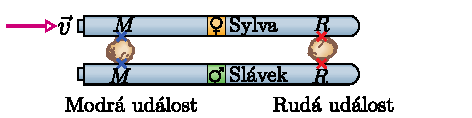
\includegraphics[width=1\linewidth]{fyz_fig0911a.pdf}}                                 \\    
        \subcaptionbox{Sylva zjišťuje vlnu od Rudé události. \label{fyz:fig0911b}}
          {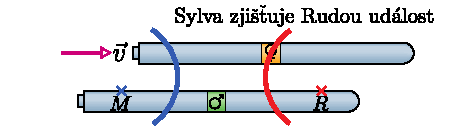
\includegraphics[width=1\linewidth]{fyz_fig0911b.pdf}}                                 \\   
        \subcaptionbox{ Slávek zjišťuje vlny od obou událostí současně. \label{fyz:fig0911c}}
          {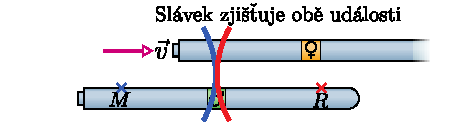
\includegraphics[width=1\linewidth]{fyz_fig0911c.pdf}} \\
        \subcaptionbox{Sylva zjišťuje vlnu od Modré události.\label{fyz:fig0911d}}
          {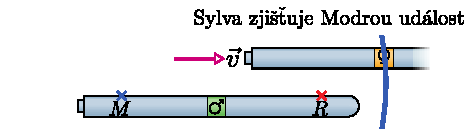
\includegraphics[width=1\linewidth]{fyz_fig0911d.pdf}}
        \caption{Kosmické lodi Sylvy a Slávka a události ze Slávkova pohledu. Sylvina loď letí 
          napravo rychlostí \(\vec{v}\). \hfill\cite[s.~1010]{Halliday2001}
        }
        \label{fyz:fig0911}
      \end{figure}
      
      Do lodí narazí dva velké meteority, jeden z nich vyvolá červenou záři (událost Rudá) a druhý
      modrou záři (událost Modrá). Tyto události nebudou nutně současné. Každá událost zanechá
      trvalou stopu na obou lodích v místech \(R\), \(R′\) a \(M\), \(M′\).

      \begin{description}[leftmargin=2em,labelindent=1em, style=nextline]
       \item [SLÁVEK řekne:] Světlo z události Rudá a světlo z události Modrá mě dostihlo ve stejném
             čase. Ze stop na své lodi jsem zjistil, že jsem stál uprostřed mezi oběma místy, z
             nichž světlo vyšlo. Události Rudá a Modrá jsou tedy současnými událostmi. 
      \end{description}
      
      Jak ale ukazuje zamyšlení nad obr. \ref{fyz:fig0911b}, rozšiřující se čelo vlny z události Rudá
      dostihne Sylvu dříve než rozšiřující se čelo vlny z události Modrá. 
      
      \begin{description}[leftmargin=2em,labelindent=1em, style=nextline]
        \item [SYLVA řekne:] Světlo z události Rudá mě dostihlo dříve než světlo z události Modrá.
              Ze stop na své lodi jsem zjistila, že i já jsem stála uprostřed mezi oběma zdroji
              světla. Události tedy nebyly současné, událost Rudá předcházela události Modrá. 
      \end{description}
        
      Tato hlášení spolu nesouhlasí. Přesto oba pozorovatelé mluví pravdu. Dobře si povšimněme, že
      je pouze jedno čelo vlny, které se šíří z místa každé události, a že toto čelo vlny se
      pohybuje stejnou rychlostí c v obou vztažných soustavách, přesně tak, jak si to žádá postulát
      rychlosti světla.

      Mohlo by se stát, že meteority by narazily do lodí takovým způsobem, že obě vzplanutí by pro
      Sylvu nastala současně. Kdyby tomu tak bylo, Slávek by je prohlásil za nesoučasná. Zkušenosti
      obou pozorovatelů jsou naprosto symetrické.
  
  \section{Relativita času}
    Jestliže pozorovatelé, kteří se vzájemně pohybují, měří časový interval (čili \emph{časovou
    odlehlost}) mezi dvěma událostmi, dojdou obecně k rozdílným výsledkům. Proč? Protože prostorová
    odlehlost událostí může ovlivnit časový interval, který pozorovatelé měří.  
    
    \begin{fyzdef}{Relativita času}{def007}
      Časový interval mezi dvěma událostmi závisí na tom, jak jsou od sebe prostorově vzdáleny, tj.
      jejich prostorové a časové odlehlosti jsou provázány.
    \end{fyzdef}

    \begin{figure}[ht!]  %\ref{fyz:fig0912}
      \centering
        \subcaptionbox{Sylva, sedící ve vlaku, měří dobu \(\Delta t_0\) mezi událostmi \(1\) a \(2\)
          jedinými hodinami \(C\) ve vlaku. Údaj hodin je ukázán dvakrát: nejprve pro událost \(1\),
          pak pro \(2\).  \label{fyz:fig0912a}}
          {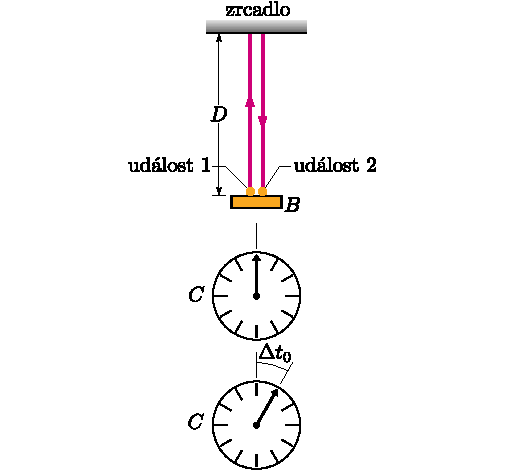
\includegraphics[width=1\linewidth]{fyz_fig0912a.pdf}}                                 \\    
        \subcaptionbox{Slávek, pozorující děj ze stanice, potřebuje dvoje synchronizované hodiny -
          \(C_1\) pro událost \(1\) a \(C_2\) pro událost \(2\). Naměří jimi dobu \(\Delta t\).
          \label{fyz:fig0912b}} 
          {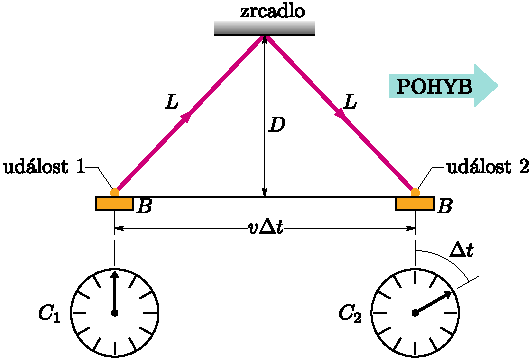
\includegraphics[width=1\linewidth]{fyz_fig0912b.pdf}}        
      \caption{Relativita času. Převzato z \cite[s.~1011]{Halliday2001}}
      \label{fyz:fig0912}
    \end{figure}

    V tomto odstavci diskutujeme uvedenou provázanost na speciálním příkladu, kdy pro jednoho z obou
    pozorovatelů jsou obě události soumístné, tj. nastávají ve stejném místě. Obecnějšími příklady
    se budeme později.

    Obr. \ref{fyz:fig0912a} ukazuje podstatu experimentu, který provádí Sylva, jež se svým vybavením
    jede vlakem konstantní rychlostí \(\vec{v}\) vzhledem k nádraží. Světelný pulz opouští světelný
    zdroj B (událost 1), pohybuje se svisle vzhůru, zrcadlo jej odráží svisle dolů a nakonec je pulz
    opět zachycen u zdroje (událost 2). Sylva naměří určitý časový interval \(\Delta t_0\) mezi
    dvěma událostmi, který je spojen se vzdáleností \(D\) od zdroje k zrcadlu vztahem
    \begin{equation}\label{fyz:eq578}
      \Delta t_0 = \frac{2D}{c} \quad \text{(Sylva)}
    \end{equation}

    V Sylvině vztažné soustavě dochází k těmto událostem v témže místě a ona potřebuje jen jedny
    hodiny \(C\) v tomto místě, aby změřila časový interval. Na obr.\ref{fyz:fig0912a} jsou hodiny
    \(C\) nakresleny dvakrát, na počátku a na konci časového intervalu.

    Uvažme nyní, jak tytéž události měří Slávek, který během průjezdu vlaku stojí na nádražním
    nástupišti. Protože Sylvino vybavení se během světelného pulzu pohybuje spolu s vlakem, Slávek
    vidí dráhu světla tak, jak je ukázána na obr. \ref{fyz:fig0912b}. Pro něho dochází k oběma
    událostem v různých místech jeho vztažné soustavy. Chce-li tedy Slávek změřit časový interval
    mezi událostmi, musí užít dvojích synchronizovaných hodin, \(C_1\) a \(C_2\), z nichž každé jsou
    na místě jedné z událostí. Podle Einsteinova postulátu rychlosti světla se světlo šířilo stejnou
    rychlostí \(c\) pro Slávka i pro Sylvu. Pro Slávka však světlo urazilo vzdálenost \(2L\) mezi
    událostmi 1 a 2. Časový interval, který Slávek mezi oběma událostmi naměřil, je
    \begin{equation}\label{fyz:eq579}
      \Delta t = \frac{2L}{c} \quad \text{(Slávek)}
    \end{equation}
    kde
    \begin{equation}\label{fyz:eq580}
      L = \sqrt{(\frac{1}{2}v\Delta t)^2 + D^2}
    \end{equation}
    Podle rov. (\ref{fyz:eq578}) můžeme \(L\) přepsat jako
    \begin{equation}\label{fyz:eq581}
      L = \sqrt{(\frac{1}{2}v\Delta t)^2 + (\frac{1}{2}c\Delta t_0)^2}
    \end{equation}
    Vyloučíme-li \(L\) z rov. (\ref{fyz:eq579}) a (\ref{fyz:eq581}) a vypočteme-li \(\Delta t\),
    dostáváme
    \begin{equation}\label{fyz:eq582}
      \boxed{\Delta t = \dfrac{\Delta t_0}{\sqrt{1  - \left(\dfrac{v}{c}\right)^2}}}
    \end{equation}

    Rov. (\ref{fyz:eq582}) nám umožňuje porovnat časové hodnoty \(\Delta t\) a \(\Delta t_0\), jak
    je změřili Slávek a Sylva. Protože \(v\) musí být menší než \(c\), musí být jmenovatel v rov.
    (\ref{fyz:eq582}) menší než jedna. Proto  \(\Delta t\) musí být větší než  \(\Delta t_0\):
    Slávek naměří větší časový interval mezi dvěma událostmi než Sylva. Slávek a Sylva změřili
    časový interval mezi týmiž dvěma událostmi, ale jejich vzájemný pohyb způsobil, že šlo o různá
    měření. Uzavíráme, že relativní pohyb může změnit tempo průběhu času mezi dvěma událostmi;
    klíčem k tomuto jevu je fakt, že rychlost světla je pro oba pozorovatele stejná.

    Rozdíl mezi Slávkovým a Sylviným měřením vyjádříme užitím následující terminologie:
    \begin{fyzdef}{Vlastní časový interval}{def004} 
      Nastávají-li dvě události na stejném místě v jisté inerciální vztažné soustavě, pak časový
      interval mezi nimi měřený v této soustavě se nazývá \textbf{vlastním časovým intervalem} nebo
      \textbf{vlastní dobou}. Měření odpovídajícího časového intervalu v jiné inerciální vztažné
      soustavě dá vždy výsledek, který je větší.
    \end{fyzdef}

    Sylva tedy měří vlastní časový interval a Slávek měří časový interval, který je větší. (Termín
    vlastní nesmíme chápat tak, že jiné měření dává nesprávný či nereálný výsledek.) Zvětšení
    časového intervalu mezi dvěma událostmi oproti vlastnímu intervalu nazýváme \textbf{dilatací
    času}\footnote{Dilatace znamená prodloužení neboli roztažení; tudíž časový interval se
    prodlužuje neboli roztahuje.}.

    Bezrozměrový podíl \(v/c\) v rov. (\ref{fyz:eq582}) značíme zpravidla jako \(\beta\cdots\)
    \textbf{rychlostním parametrem}. Je to tedy rychlost vyjádřená jako zlomek rychlosti světla.
    Bezrozměrovou převrácenou hodnotu odmocniny v rov. (\ref{fyz:eq582}) značíme často jako
    \(\gamma\) a nazýváme \textbf{Lorentzovým faktorem}.
    \begin{equation}\label{fyz:eq583}
      \boxed{\gamma = \dfrac{1}{\sqrt{1-\beta^2}}}
    \end{equation}
    S těmito označeními můžeme přepsat rov. (\ref{fyz:eq582}) jako
    \begin{equation}\label{fyz:eq584}
      \boxed{\Delta t = \gamma \delta t_0} \quad\text{dilatace času}
    \end{equation}

    Rychlostní parametr \(\beta\) je vždy menší než jedna, a pokud \(v\) není rovno nule, je
    \(\gamma\) vždy větší než jedna. Rozdíl mezi \(\gamma\) a \(1\) však není výrazný, dokud neplatí
    \(v > \num{0.1}c\). Takže \emph{„stará relativita“} je docela dobře použitelná pro \(v <
    \num{0.1}c\), ale pro větší hodnoty v musíme užít speciální relativity. Jak ukazuje obr.
    \ref{fyz:fig0913}, velikost γ prudce roste, když se \(\beta\) blíží jedné (čili \(v\) se blíží k
    \(c\)). Čím je tedy větší relativní rychlost mezi Sylvou a Slávkem, tím větší je časový interval
    měřený Slávkem, až pro dostatečně velkou rychlost se prodlouží téměř ve věčnost.

    Můžeme se ptát, co řekne Sylva na to, že Slávek naměřil větší časový interval, než jaký naměřila
    ona. Nebude to pro ni žádným překvapením, protože podle ní Slávek nesynchronizoval své hodiny
    \(C_1\) a \(C_2\), ačkoli tvrdí, že to učinil. Připomeňme, že pozorovatelé pohybující se vůči
    sobě se neshodují v tom, co je současné. Slávek tedy tvrdí, že obojí jeho hodiny ukazovaly
    současně stejný čas v době, kdy nastala událost 1. Podle Sylvy však byly Slávkovy hodiny \(C_2\)
    nesprávně nastaveny. Když tedy na nich Slávek odečítal čas události 2, zaznamenal podle Sylvy
    příliš velký čas, a proto připsal oběma událostem větší časový interval než Sylva.

    \luagraphic[1]{fyz_fig0913.pdf}{Lorentzův faktor \(\gamma\) jako funkce rychlostního parametru 
    \(\beta = v/c\). \cite[s.~1013]{Halliday2001}}{fyz:fig0913}

    \subsection{Dva testy dilatace času}
      \textbf{Mikroskopické hodiny}: Subatomární částice zvané miony jsou nestabilní. To znamená, že
      \emph{mion} se v krátké době po svém vzniku \emph{rozpadne}\footnote{přemění na částice jiných
      typů}. \emph{Doba života} mionu je časový interval mezi jeho vznikem (událost 1) a jeho
      rozpadem (událost 2). Jsou-li miony v klidu a jejich doby života jsou měřeny nehybnými
      hodinami (např. v laboratoři), pak jejich průměrná doba života je \SI{2 200}{\micro\sec}. Je
      to vlastní časový interval, protože pro každý mion nastávají události 1 a 2 v témže místě ve
      vztažné soustavě mionu. Tento vlastní časový interval označíme \(\Delta t_0\) a vztažnou
      soustavu, v níž bylo provedeno měření, nazveme klidovou soustavou mionu. Pokud se však miony
      pohybují (např. vůči laboratoři), pak měření jejich dob života provedené laboratorními
      hodinami povede k větší (dilatované) průměrné době života. Pro potvrzení tohoto závěru byla
      provedena měření průměrné doby života mionů pohybujících se rychlostí \(num{0.999 4}c\)
      vzhledem k laboratorním hodinám. Z rov. (\ref{fyz:eq583}) s \(\beta = \num{0.999 4}\) lze
      obdržet pro tuto rychlost Lorentzův faktor
      \begin{equation*}
        \gamma = \dfrac{1}{\sqrt{1-\beta^2}} = \dfrac{1}{\sqrt{1-\num{0.999 4}^2}} = \num{28.87},
      \end{equation*}
      což je podstatně větší než jedna. Rov. (\ref{fyz:eq584}) pak dává pro průměrnou dilatovanou
      dobu života
      \begin{equation*}
        \Delta t = \gamma\Delta t_0=\num{28.87}\cdot\SI{2 200}{\micro\sec}=\SI{63.5}{\micro\sec},
      \end{equation*}
      Skutečně pozorovaná hodnota potvrdila tento výsledek v mezích pozorovacích chyb.

      \textbf{Makroskopické hodiny}: V říjnu 1977 Joseph Hafele a Richard Keating uskutečnili
      vskutku ohromující experiment. Nechali čtvery přenosné atomové hodiny dvakrát obletět kolem
      světa na komerčních leteckých linkách; každé z nich v jiném směru. Cílem bylo \emph{„testovat
      Einsteinovu teorii relativity pomocí makroskopických hodin“}. Jak jsme právě viděli, předpověď
      časové dilatace podle Einsteinovy teorie byla potvrzena v mikroskopickém měřítku, ale něco
      docela jiného je vidět potvrzení na skutečných hodinách. Taková makroskopická měření byla
      umožněna pouze velmi vysokou přesností moderních atomových hodin. Hafele a Keating ověřili
      předpovědi teorie s přesností 10 \%. (Einsteinova obecná teorie relativity, která předpovídá,
      že tempo chodu hodin je ovlivněno gravitací, hraje v daném experimentu rovněž roli.) 
      
      O několik let později fyzikové z univerzity v Marylandu provedli podobný experiment se
      zvýšenou přesností. Oblétali s atomovými hodinami Chesapeakskou zátoku stále dokola po dobu 15
      h a podařilo se jim potvrdit předpověď časové dilatace s přesností lepší než 1 \%. Když se
      dnes atomové hodiny přenášejí z jednoho místa na druhé kvůli kalibraci či z jiných důvodů,
      bere se vždy ohled na časovou dilataci způsobenou jejich pohybem.

      %--relativistický nákladní vagon řítící se kolem nás------------
      % !TeX spellcheck = cs_CZ
\begin{mdframed}[style=mdexam]
  \begin{example}\label{fyz:fey_exam020}
    Stojíme u železničních kolejí, když nás náhle vyděsí relativistický nákladní vagon řítící se
    kolem nás, jak je ukázáno na obrázku. Ve vagonu je dobře vybavený hobo (americký železniční
    tulák) Jack, který posílá laserový pulz od přední k zadní stěně vagonu. (a) Dá naše měření
    rychlosti pulzu větší, menší, nebo stejný výsledek jako měření Jackovo? (b) Je Jackovo měření
    doby letu pulzu měřením vlastního času? (c) Jsou Jackova a naše měření doby letu pulzu spojena
    rov. (\ref{fyz:eq584})?

    {\centering
    \captionsetup{type=figure}
    \luafigure[1]{fyz_fig914.pdf}
    \captionof{figure}{K příkladu \ref{fyz:fey_exam020}. (\cite[s.~1013]{Halliday2001})
    \label{fyz:fig914}}
    \par}  
  \end{example}
\end{mdframed}
      %---------------------------------------------------------------

      %--hvězdolet míjí Zemi relativní rychlostí 0,999 0c-------------
      % !TeX spellcheck = cs_CZ
\begin{mdframed}[style=mdexam]
  \begin{example}\label{fyz:fey_exam021}
    Náš Hvězdolet míjí Zemi relativní rychlostí \(\num{0.999 0}c\). Po uplynutí \num{10.0} roků se
    zastavíte na pozorovatelně LP13 a pak cestujeme zpět k Zemi stejnou relativní rychlostí. Cesta
    zabere dalších \num{10.0} roků (našeho času). Jak dlouho trvá cesta podle měření vykonaných na
    Zemi? (Zanedbejme jakýkoli vliv způsobený zrychlením během zastavování a rozletu.)
    
    \vspace{1em}
    Začátek i konec cesty tam (Země - LP13) nastávají ve naší vztažné soustavě, tj. ve vašem
    hvězdoletu, na stejném místě. Měříme tedy vlastní čas \(\Delta t_0\) cesty, který je určen jako
    \(\num{10.0} y\). Rov. (\ref{fyz:eq582}) dává odpovídající čas \(\Delta t\), jak je naměřen v
    pozemské vztažné soustavě
    \begin{align*}
      \Delta t &= \dfrac{\Delta t_0}{\sqrt{1  - \left(\dfrac{v}{c}\right)^2}}
                = \dfrac{\num{10.0} y}{\sqrt{1  - (\num{0.999 0}c/c)^2}}      \\
               &= \num{22.37}\cdot\num{10.0} y = \num{224} y
    \end{align*}
    Při cestě zpět (LP13 - Země) máme stejnou situaci a stejné údaje. Celková cesta tedy zabere 20
    roků vašeho času, ale
    \begin{equation*}
      \Delta t_{celk}  = 2\cdot\num{224} y = \num{448} y
    \end{equation*}
    pozemského času. Jinými slovy, zestárli jsme o \num{20} let, zatímco Země zestárla o \num{448}
    let. Ačkoli nelze (pokud dnes víme) cestovat do minulosti, není vyloučeno cestování např. do
    budoucnosti Země pomocí velmi rychlého relativního pohybu, který změní tempo plynutí času.
  \end{example}
\end{mdframed}
      %---------------------------------------------------------------

      %--doba života kaonu--------------------------------------------
      \begin{fyzexam}{Elementární částice nazvaná kladný kaon (\(K^+\)) má v klidu průměrnou dobu života
  \protect\SI{0.1237}{\protect\micro\protect\s}, tj. jedná se o dobu života měřenou v klidové
  soustavě kaonu. Vytvářejí-li se v atmosféře kladné kaony s rychlostí \num{0.990}c vzhledem k
  zemské vztažné soustavě, jak daleko se v této soustavě během své doby života dostanou?
  \cite[s.~1014]{Halliday2001}}{exam022} 

  \vspace{1em}
  V soustavě pozorovatele na Zemi je vzdálenost \(d\) uražená kaonem spojena s jeho rychlostí \(v =
  \num{0.990}c\) a dobou jeho letu \(\Delta t_k\) vztahem \(d = v\Delta t_k\). (Toto tvrzení není
  ovlivněno relativitou, protože všechny veličiny se měří v téže vztažné soustavě.) Kdybychom
  neužívali speciální relativity, doba letu by činila \SI{0.1237}{\micro\s}, což je doba života
  částice, a tudíž uražená vzdálenost by byla
  \begin{align*}
    d &= v\Delta t_k                                                        \\
      &= \num{0.990}\cdot\SI{3.00e8}{\m\per\s}\cdot\SI{1.237e-7}{\s}        \\
      &= \SI{36.7}{\m}  \qquad\text{(chybná odpověď)} 
  \end{align*}  
  Je však třeba užít speciální relativity a doba letu kaonu v laboratorní soustavě je jeho
  dilatovaná doba života \(\Delta t\). Podle rov. (\ref{fyz:eq582}) můžeme najít \(\Delta t\) ze
  znalosti vlastní doby života kaonu \(t_0 = \SI{0.1237}{\s}\) měřené v jeho klidové soustavě
  \begin{align*}
    \Delta t &= \dfrac{\Delta t_0}{\sqrt{1  - \left(\dfrac{v}{c}\right)^2}}   \\
              &= \dfrac{\SI{0.123 7e-6}{\s}}{\sqrt{1  - (\num{0.990}c/c)^2}}  \\
              &= \SI{8.769e-7}{\s}
  \end{align*}
  To je sedmkrát větší než vlastní doba života kaonu. (Tento výpočet přihlížel k relativitě, protože
  jsme museli přepočítat data z klidové soustavy částice do soustavy laboratorní.) Nyní najdeme
  délku cesty kaonu v laboratorní soustavě jako
  \begin{align*}
    d &= v\Delta t_k                                                      
      = \num{0.990}\cdot\SI{3.00e8}{\m\per\s}\cdot\SI{8.769e-7}{\s}        \\
      &= \SI{260}{\m}  
  \end{align*} 

  {\centering
  \captionsetup{type=figure}
  \luafigure[0.8]{fyz_fig0915.png}
  \captionof{figure}{Kaon v atmosféře Země žije déle, jak je měřeno pozorovatelem vázaným na Zemi,
              než měřeno vnitřními hodinami kaonu. (\cite[s.~1013]{Halliday2001})
              \label{fyz:fig0915}} \par}  

  Tato vzdálenost je sedmkrát větší než podle naší první (nesprávné) odpovědi. Experimenty tohoto
  druhu, které ověřují speciální relativitu, jsou už po desetiletí pro fyzikální laboratoře
  rutinní záležitostí.    
\end{fyzexam}
      %---------------------------------------------------------------
  
  \section{Relativita délky}\label{fyz:IchapXVsecII}     
    Chceme-li měřit délku tyče, která je vůči nám v klidu, můžeme zaznamenat polohy jejich konců na
    dlouhém nehybném měřítku a oba údaje odečíst. Pokud se ale tyč pohybuje, musíme zaznamenat
    polohy koncových bodů současně (v naší vztažné soustavě). Jinak by se naše měření nemohlo
    nazývat měřením délky. Obr. 38.7 naznačuje potíže, na něž narážíme, když chceme změřit délku
    pohybujícího se tučňáka zaznamenáním polohy jeho hrudi a zad v rozdílných časech. Protože
    současnost je relativní a ovlivňuje měření délky, je i délka relativní veličinou.  

    Nechť \(L_0\) je délka tyče, kterou měříme, když je tyč v klidu (za předpokladu, že my i tyč
    jsme v téže vztažné soustavě, klidové soustavě tyče). Jestliže se naopak tyč vzhledem k nám
    pohybuje rychlostí \(v\) ve směru délky tyče, naměříme délku \(L\) danou vztahem pro
    \textbf{kontrakci délek}:
    \begin{equation}\label{fyz:eq997}
      L = L_0\sqrt{1-\beta} = \dfrac{L_0}{\gamma}
    \end{equation}
    Protože Lorentzův faktor \(\gamma\) je při relativním pohybu vždy větší než jedna, je \(L\) vždy
    menší než \(L_ 0\). Relativní pohyb způsobuje \textbf{kontrakci délky} a \(L\) se nazývá
    \emph{kontrahovaná délka}. Protože \(\gamma\) s rychlostí v roste, roste s relativní rychlostí i
    kontrakce délky.

    \begin{tcnote}
      Délka objektu \(L_0\) měřená v jeho klidové soustavě je \emph{vlastní délka} čili
      \emph{klidová délka}. Měření délky v každé vztažné soustavě, která koná relativní pohyb
      rovnoběžný s touto délkou, dává výsledek, který je vždy menší než vlastní délka.
    \end{tcnote}

    Pozor: kontrakce délky nastává pouze ve směru relativního pohybu. Dodejme, že měřená délka
    nemusí být délkou objektu, jako je tyč či obruč. Může to být i délka (či vzdálenost) mezi dvěma
    objekty v téže klidové soustavě - například vzdálenost Slunce a blízké hvězdy (které jsou
    alespoň přibližně vůči sobě v klidu).

    Zkracuje se objekt opravdu? Realita je založena na pozorováních a měřeních; jestliže výsledky
    vždy vzájemně souhlasí a nelze najít žádnou chybu,pak to,co bylo pozorováno a měřeno, je reálné.
    V tomto smyslu se objekt opravdu zkracuje. Přesněji bychom však mohli říci, že zkrácení objektu
    je opravdu změřeno - pohyb ovlivňuje měření a tím i realitu.
    
    Musí blesková fotografie ukázat zkrácení objektu? Nikoli, protože není pořízena zachycením
    světla, které objekt emitoval v určitém okamžiku (současně). Zaznamenává světlo z objektu, které
    dospělo do kamery v okamžiku expozice filmu, bez ohledu na to, kdy bylo emitováno.

    \begin{figure}[ht!]  %\ref{fyz:fig0098}
      \centering
      \subcaptionbox{\label{fyz:fig0957a}}{\luafigure[0.8]{fyz_fig0957a.pdf}}              \\                                                   
      \subcaptionbox{\label{fyz:fig0957b}}{\luafigure[0.8]{fyz_fig0957b.pdf}}
      \caption{Chceme-li měřit délku pohybujícího se tučňáka měřením polohy jeho hrudi a zad, 
               musíme je měřit současně (v naší vztažné soustavě). Tak je tomu v (a), ale nikoli v 
               (b). \cite[s.~1015]{Halliday2001}}
      \label{fyz:fig0957}
    \end{figure}

    Měříme-li zkrácenou délku, například délku tyče, co řekne o našem měření pozorovatel pohybující
    se spolu s tyčí? Podle něho jsme nezaznamenali polohu obou konců tyče současně. (Připomeňme, že
    pozorovatelé ve vzájemném pohybu se neshodují v tom, co je současné.) Z hlediska zmíněného
    pozorovatele jsme nejprve zaznamenali polohu předního konce tyče a teprve o něco později polohu
    zadního konce. Proto jsme změřili délku, která je menší než vlastní délka.

    \subsection{Odvození vzorce pro kontrakci délek}\label{fyz:IchapXVsecIIssecI}  
      Kontrakce délky \eqref{fyz:eq997} přímo souvisí s dilatací času. Uvažujme ještě jednou naše
      dva pozorovatele. Sylva, která sedí ve vlaku projíždějícím nádražím, stejně jako Slávek, který
      stojí na nástupišti, chtějí změřit délku nástupiště. Slávek užije plátěného metru a zjistí
      délku \(L_0\). Je to vlastní délka, protože nástupiště je vzhledem k němu vklidu. Slávek také
      zjišťuje, že Sylva ve vlaku projede kolem této délky za čas \(\Delta t = \frac{L_0}{v}\), kde
      \(v\) je rychlost vlaku. Je tedy
      \begin{equation}\label{fyz:eq998}
        L_0 = v\Delta t \qquad\text{Slávek}
      \end{equation}
      Časový interval \(\Delta t\) není vlastním časovým intervalem, protože dvě události, které jej
      ohraničují (Sylvino míjení začátku a konce nástupiště), nastávají ve dvou různých místech a
      Slávek musí užít dvojích synchronizovaných hodin, aby interval \(\Delta t\) změřil. 
      
      Pro Sylvu se však nástupiště pohybuje. Zjišťuje, že obě události, které měřil Slávek,
      nastávají v \emph{témže místě} v její vztažné soustavě. Může jim přiřadit čas pomocí jediných
      nehybných hodin, takže interval \(\Delta t_0\), který měří, je vlastní časový interval. Pro
      ni je délka nástupiště \(L\) dána vztahem
      \begin{equation}\label{fyz:eq999}
        L = v\Delta t_0 \qquad\text{Sylva}
      \end{equation}

      Vydělíme-li rov. \eqref{fyz:eq999} rovnicí \eqref{fyz:eq998} a užijeme pro dilataci času
      rov. \eqref{fyz:eq584}, dostaneme
      \begin{align}
        \dfrac{L}{L_0} &= \dfrac{v\Delta t_0}{v\Delta t} = \dfrac{1}{\gamma} \nonumber \\
        \shortintertext{neboli}
        L              &= \dfrac{L_0}{\gamma}                   \label{fyz:eq1000}
      \end{align}
      což je rov. \eqref{fyz:eq997} pro kontrakci délky.
    
      %--Relativita délky---------------------------------------------
      \begin{fyzexam}{Na obr.38.8 se Sylva (v bodě \(A\)) a Slávkova kosmická loď (o vlastní délce \(L_0 =
  \SI{230}{\m}\)) míjejí konstantní relativní rychlostí \(v\). Sylva měří časový
  interval \SI{3.57}{\micro\s}, po který ji loď míjí (od průchodu bodu \(B\) do průchodu
  bodu \(C\)). Jaký je rychlostní parametr \(β\) mezi Sylvou a lodí?
  \hfill\cite[s.~1015]{Halliday2001}}{exam018} 

  {\centering
  \captionsetup{type=figure}
  \luafigure[0.8]{fyz_fig0958.pdf}
  \captionof{figure}{Příklad \ref{fyz:exam018}. Sylva měří, jak dlouho trvá lodi, když ji
    v bodě A míjí. (\cite[s.~1016]{Halliday2001})
    \label{fyz:fig0958}
  } 
  \par} 

\end{fyzexam}
      %---------------------------------------------------------------

  \section{Princip relativity}\label{fyz:IchapXVsecIII}     
    Newton byl první, kdo vyslovil \emph{princip relativity} jako jeden z důsledků pohybových
    zákonů: Vzájemné pohyby těles, nacházejících se v daném prostoru, jsou stejné ať je prostor v
    klidu, nebo se pohybuje rovnoměrně přímočaře vpřed. To například znamená, že jestliže se
    kosmická loď pohybuje rovnoměrnou rychlostí, všechny experimenty a všechny jevy v lodi budou
    probíhat tak, jakoby se loď nepohybovala (samozřejmě za předpokladu, že se nikdo nebude dívat
    ven). To je smyslem principu relativity. Myšlenka je jednoduchá, jedinou otázkou je, zda je
    pravda, že ve všech experimentech provedených v pohybující se soustavě budou všechny fyzikální
    zákony stejné, jako v soustavě, která je v klidu. Nejprve zjistíme, zda v pohybující se soustavě
    mají Newtonovy zákony stejný tvar.

    \luagraphic[0.8]{fyz_fig0005.pdf}{Dvě souřadnicové soustavy v rovnoměrném relativním pohybu
      podél svých x-ových os. (\cite[s.~211]{Feynman01})}{fyz:fig0005}
  
    Předpokládejme, že se Pavel pohybuje konstantní rychlostí \(u\) ve směru osy \(x\), přičemž měří
    polohu určitého budu (obr. \ref{fyz:fig0005}). Ve své souřadnicové soustavě si značí souřadnici
    ve směru osy \(x\) jako \(x'\). Petr je v klidu, přičemž měří polohu téhož bodu. Souřadnici ve
    směru osy \(x\) ve své souřadnicové soustavě značí jako \(x\). Počátek souřadnicové soustavy, v
    níž je Pavel, se posune za čas \(t\) o vzdálenost \(ut\), a jestliže soustavy z počátku
    splývaly, máme
    \begin{equation}\label{fyz:eq183}
      x' = x - ut, \quad y' = y, \quad z' = z, \quad t' = t. 
    \end{equation}
    Dosadíme-li tuto transformaci do Newtonových zákonů, zjistíme, že se přetransformovaly do
    stejných zákonů v čárkované soustavě. To znamená, že Newtonovy zákony mají stejný tvar v
    pohybující se soustavě jako v stacionární soustavě, a proto na základě mechanických experimentů
    není možné říci, zda se soustava pohybuje či nikoliv (což jsme ukázali v kapitole
    \ref{vol02:fyz:IchapXIsecI}). 
    
    Zájem o tento princip vzrostl v minulém století v důsledku výzkumu elektrických, magnetických a
    světelných jevů, jež vyústilo v \emph{Maxwellovu teorii elektromagnetického pole}, která
    jednotně popisuje elektřinu, magnetizmus a světlo. Zdálo se však, že Maxwellovy rovnice
    nevyhovovaly \emph{principu relativity}, neboť přetransformujeme-li Maxwellovy rovnice pomocí
    rovnic \ref{fyz:eq183}, nebudou mít stejný tvar. Proto by se elektrické a optické jevy v letící
    kosmické lodi měli lišit od jevů v nehybné lodi. Těmito jevy by pak bylo možné určit rychlost
    lodi, a ve speciálním případě pomocí vhodných optických nebo elektrických měření by bylo možné
    určit i absolutní rychlost lodi. Jedním z důsledků Maxwellových rovnic je, že dojde-li k určité
    poruše pole, při níž vniká světlo, toto elektromagnetické vlnění se šíří všemi směry stejnou
    rychlostí \(c = \SI{3e5}{\km\per\s}\). Dalším důsledkem těchto rovnic je, že pohybuje-li se
    zdroj poruchy, šíří se vyzářené světlo prostorem stejnou rychlostí \(c\). Tato nezávislost
    pohybu vlnění na pohybu zdroje vede k zajímavému problému:
    
    Předpokládejme, že sedíme v autě, jež jede rychlostí \(u\) a že světlo z reflektorů auta za 
    námi nás míjí rychlostí \(c\). Zdiferencováním první rovnice \ref{fyz:eq183} máme
    \begin{equation}\label{fyz:eq184}
      \der{x'}{t} =\der{x}{t} - u, 
    \end{equation}       
    což znamená, že podle \emph{Galileovy transformace} by zdánlivá rychlost světla měřená z auta
    nemohla být \(c\), ale \(c-u\). Tato představa byla v souladu s \textbf{vlnovou teorií světla},
    podle které světlo bylo chápáno jako vlnění všudypřítomného média - \emph{etheru}.  O začlenění
    etheru do přírodních věd se postarali v sedmnáctém století Rene Descartes a Ch. Huyghens se svou
    vlnovou teorií světla, ale jejich názory byly dočasně převáženy autoritou Isaaka Newtona, který
    prezentoval světlo jako proud částic (fotonů), šířících se prázdným prostorem. Od počátku 19.
    století byla vlnová povaha světla jednoznačně prokázána difrakčními jevy a díky tomu se ve vědě
    znovu rozšířila myšlenka tzv. světlonosného éteru, které dala formální rámec Maxwellova teorie
    světla a elektromagnetického pole.  
    
    \begin{tcnote}        
      Vznik a zdokonalení vlnové teorie světla se datuje o několik desítek let dříve, než byla
      prokázána elektromagnetická podstata světelných vln. Pro pionýry optiky bylo přirozené
      uvažovat světelné vlny jako vlnění všudypřítomného pružného prostředí, zvaného ether, a díky
      úspěšnému vysvětlení difrakčních a interferenčních jevů pomocí etherových vln se stal pojem
      etheru běžný a jeho existence nepochybná. Maxwellova elektromagnetická teorie světla z roku
      1864 a její experimentální potvrzení Hertzem v roce 1887 zbavilo ether většiny jeho
      vlastností, avšak nikdo v té době ještě nebyl patrně ochoten zavrhnout základní myšlenku,
      reprezentovanou etherem, totiž že světlo se šíří vzhledem k nějaké univerzální vztažné
      soustavě. Ukažme si na příkladu pomocí jednoduché analogie, co tato myšlenka ve svých
      důsledcích znamená.
    \end{tcnote}

    Na myšlence, že se světlo šíří různou rychlostí, bylo založeno mnoho experimentů k určení
    rychlosti Země, ale všechny selhaly - nedávaly vůbec žádné rychlosti. Ukázalo se, že někde
    \emph{byla} chyba, a sice něco nebylo v pořádku s fyzikálními rovnicemi. Co to asi mohlo být?

    \subsection{Problém volby vztažné soustavy}
      Zmínili jsme se již o úloze etheru jako o univerzální vztažné soustavě, vůči níž se měly
      světelné vlny šířit. Kdykoli mluvíme o \emph{„pohybu"}, máme samozřejmě vždy na mysli
      \emph{„pohyb vůči vztažné soustavě"}. Vztažnou soustavou může být silnice, zemský povrch,
      Slunce, střed naší galaxie, avšak v každém případě ji musíme specifikovat. Kameny padají na
      Bermudách i v australském Perthu „dolů" a přesto se pohybují vzájemně právě opačnými směry
      vzhledem ke středu Zeme. Jak v této situaci volit správnou vztažnou soustavu? Spojit ji s
      povrchem Zeme nebo s jejím středem? Odpověď zní, že jsou správné všechny vztažné soustavy, i
      když v konkrétním případě může být jedna z nich vhodnější k popisu než ostatní. Kdyby
      existoval klidný ether vyplňující celý prostor, mohli bychom k němu vztahovat každý pohyb a
      obyvatelé Bermud a Perthu by se nemuseli divit. Z neexistence etheru však plyne, že
      \textbf{neexistuje ani žádná univerzální vztažná soustava}, takže existuje pohyb výhradně jen
      vůči pozorovateli nebo jeho přístroji. Když se díváme z koše volného balónu, vznášejícího se
      nad souvislou oblačnou pokrývkou, na jiný volný balón, jak mění vůči nám polohu, nemůžeme
      nijak zjistit, který balón se „skutečně" pohybuje (obr. \ref{fyz:fig0905}). Kdybychom byli
      izolováni ve vesmíru, nemohli bychom žádným způsobem zjistit, pohybujeme-li se či ne, neboť
      bez vztažné soustavy ztrácí pojem pohybu smysl.

      \luagraphic[1]{fyz_fig0905.png}{Každý pohyb je relativní vzhledem k pozorovateli. 
      (\cite[s.~24]{Beiser1975})}{fyz:fig0905}

      Teorie relativity vznikla z rozboru fyzikálních důsledků neexistence univerzální vztažné
      soustavy. Speciální teorie relativity, formulovaná Albertem Einsteinem v roce 1905, se zabývá
      \textbf{inerciálními vztažnými soustavami}, což jsou vztažné soustavy pohybující se navzájem
      konstantní rychlostí\footnote{Konstantní rychlostí se zde i všude v dalším textu míní
      konstantní rychlost jako vektor, tj. u pohybu s konstantní rychlostí jde o pohyb rovnoměrný
      přímočarý.}. Obecná teorie relativity, předložená Einsteinem o deset let později, zahrnuje i
      problémy vztažných soustav pohybujících se navzájem se zrychlením. Pozorovatel, uzavřený v
      izolované laboratoři, může zjistit zrychlení; to z vlastní zkušenosti potvrdí každý, kdo jel
      výtahem nebo na kolotoči. Speciální teorie relativity měla hluboký vliv na celou fyziku a
      budeme se jí zabývat v této kapitole, dříve než přikročíme ke stručnému nástinu obecné teorie
      relativity.

      Speciální teorie relativity spočívá na dvou postulátech. První z nich tvrdí: 
      \begin{fyzdef}{První postulát STR}{def008}
        Všechny fyzikální zákony lze vyjádřit rovnicemi, jež mají stejný tvar ve všech vztažných
        soustavách pohybujících se navzájem konstantní rychlostí. 
      \end{fyzdef}
      Tento postulát vyjadřuje neexistenci univerzální vztažné soustavy. Kdyby měly fyzikální zákony
      různý tvar pro různé, navzájem se pohybující pozorovatele, bylo by možné z těchto rozdílů
      určit, které objekty v prostoru \emph{„stojí"} a které se \emph{„pohybují"}. Protože však
      žádná univerzální vztažná soustava neexistuje, neexistuje v přírodě ani možnost takového
      rozlišení; proto uvedený postulát.

      Druhý postulát speciální teorie relativity říká:
      \begin{fyzdef}{Druhý postulát STR}{def009}
        Rychlost světla ve vakuu má pro všechny pozorovatele stejnou hodnotu, bez ohledu na jejich 
        pohybový stav. 
      \end{fyzdef}
      Tento postulát plyne přímo z výsledku Michelsonova-Morleyova pokusu (kapitola
      \ref{fyz:IchapXVsecV}) a dalších experimentů.

      Na první pohled tyto postuláty nevypadají nijak převratně. Ve skutečnosti boří téměř všechny
      intuitivní pojmy prostoru a času, které si vytváříme z každodenní zkušenosti. Pro ilustraci
      jednoduchý příklad. 
      %--Člun na řece světlice----------------------------------------
      % !TeX spellcheck = cs_CZ
\begin{mdframed}[style=mdexam]
  \begin{example}\label{fyz:fey_exam017}
    Na obr. \ref{fyz:fig0906a} máme ještě jednou dva čluny \(A\) a \(B\), z nichž člun \(A\) stojí na
    místě, kdežto Člun \(B\) se pohybuje konstantní rychlostí \(v\). Nad vodou je hustá mlha, a tak
    pozorovatelé na obou člunech nemohou vědět, který z nich je v pohybu. V okamžiku, kdy je člun
    \(A\) těsně u člunu \(B\), zapálí světlici. Světlo se z ní šíři rovnoměrně všemi směry, podle
    druhého postulátu speciální teorie rela­tivity. Podle prvého postulátu speciální teorie
    relativity musí každý pozorovatel na svém Člunu vidět šířící se světelnou kouli, v jejímž středu
    je on sám, přestože jeden z nich mění svou polohu vůči místu, kde vzplanula světlice.
    Pozorovatelé ovšem nemohou zjistit, který z nich se takto pohybuje, neboť mlha vylučuje
    jakoukoli vztažnou soustavu, kromě soustav pevně spojených s každým člunem, a jelikož je
    rychlost světla pro oba stejná, musí být pozorování na obou člunech naprosto shodná.

    {\centering
    \captionsetup{type=figure}
    \luafigure[1]{fyz_fig0906a.png}
    \captionof{figure}{Relativistické jevy se liší od našich běžných zkušeností.
    \cite[s.~25]{Beiser1975}
    \label{fyz:fig0906a}}
    \par}
    \vspace{1em}

    Proč je situace na obr. \ref{fyz:fig0906a} neobvyklá? Uvažujme známější analogickou situaci. Je
    jasný den, čluny jsou na moři a někdo z posádky jednoho člunu hodí do vody kámen právě v
    okamžiku, kdy jsou bok po boku. Na vodě se začnou šířit známé kruhy jako na obr.
    \ref{fyz:fig0906b}, které se však jeví dvěma pozorovatelům na dvou různých člunech různě. Už jen
    na základě zjištění, zda je nebo není ve středu těchto kruhů, může každý pozorovatel říci,
    pohybuje-li se vůči vodě či nikoliv. Voda je sama o sobě vztažnou soustavou a pozorovatel na
    člunu, který se vůči ní pohybuje, měří rychlost kruhů vzhledem k sobě samotnému; ta je v různých
    směrech různá, na rozdíl od rychlosti kruhů, měřené pozorovatelem na nehybném člunu. Je důležité
    si uvědomit, že pohyb a vlny ve vodě jsou úplně jiné než pohyb a vlny v (prázdném) prostoru;
    zatímco samotná voda je vztažnou soustavou, prostor takovou soustavou být nemůže, a rychlost
    šíření vln na vodě se na rozdíl od rychlosti šíření světelných vln v prostoru mění s pohybem
    pozorovatele.

    {\centering
    \captionsetup{type=figure}
    \luafigure[1]{fyz_fig0906b.png}
    \captionof{figure}{Analogická situace, šíření kruhů na vodní hladině.
    \cite[s.~25]{Beiser1975}
    \label{fyz:fig0906b}}
    \par}
    \vspace{1em}

  \end{example}
\end{mdframed}
      %---------------------------------------------------------------

    
  %----------------------- Lorentzova transformace -------------------------------------------------
  \section{Lorentzova transformace}\label{fyz:IchapXVsecIV}
    Když se zjistilo, že s rovnicemi v uvedeném případě není vše v pořádku, nejprve padlo podezření 
    na Maxwellovy rovnice elektrodynamiky, jež byly tehdy známy jen dvacet let. Zdálo se být téměř 
    samozřejmé, že tyto rovnice musí byt nesprávné a proto byla snaha je změnit tak, aby při 
    Galileiho transformaci zachovávaly princip relativity. Přitom bylo třeba do těchto rovnic 
    zavést nové členy, jež vedly k předpovědi nových elektrických jevů, jejichž existence se 
    experimentálně nepotvrdila. Proto bylo třeba tuto cestu opustit. Postupně se pak stalo zřejmým, 
    že Maxwellovy zákony elektrodynamiky jsou správné a zdroj problému je třeba hledat někde 
    jinde.  
    
    Mezitím si \emph{H. A. Lorentz} všiml pozoruhodné věci, když použil v Maxwellových rovnicích
    substituci
    \begin{gather}\label{fyz:eq185}
      x' = \frac{x - ut}{\sqrt{1-\dfrac{u^2}{c^2}}}, \;
      \begin{array}{c}      
        y' = y, \\ z' = z,                         
      \end{array}\;
      t' = \frac{t-\dfrac{u}{c^2}x}{\sqrt{1-\dfrac{u^2}{c^2}}}. 
    \end{gather} 
    tvar rovnic se nezměnil. Rovnice \ref{fyz:eq185} jsou známé jako \emph{Lorentzovy 
    transformace}. Einstein sledoval původní \emph{Poincarého} myšlenku a pak navrhl, že všechny 
    fyzikální zákony, by měly být takové, aby se při Lorentzově transformaci neměnily. Jinými 
    slovy, měly bychom změnit ne zákony elektrodynamiky, ale zákony mechaniky. Jak se ukázalo 
    jediné co je třeba, je změnit hmotnost \(m\) v Newtonových rovnicích podle vztahu 
    \ref{fyz:eq182}. Po této změně budou Newtonovy zákony v souladu se zákony elektrodynamiky. Když 
    k porovnání Pavlových a Petrových měření použijeme Lorentzovu transformaci, nikdy nebudeme 
    schopni zjistit, zda se jeden nebo druhý pohybuje, neboť tvary všech rovnic budou v obou 
    souřadnicových soustavách stejné. 
    
    Pro pochopení smyslu této nové transformace nestačí studovat jen zákony mechaniky, ale podobně 
    jako Einstein, musíme provést analýzu našeho chápání prostoru a času. 

    Ukažme si na příkladu pomocí jednoduché analogie, co tato myšlenka ve svých důsledcích znamená.
    %--Člun na řece-------------------------------------------------
    \begin{fyzexam}{Představme si, že pozorujeme dva čluny na řece. Obrázek 1.1 znázorňuje řeku šířky
  \(L\), která teče rychlostí \(v\). Dva čluny startují od téhož břehu řeky stejně velkou rychlostí
  \(V\). Člun \(A\) přepluje řeku do místa na druhém břehu přímo naproti výchozímu bodu, a poté se
  vrátí, zatímco člun \(B\) pluje po proudu na vzdálenost \(L\) a rovněž se vrátí. Vypočítejme dobu,
  potřebnou na obě cesty tam a zpět. \hfill\cite[s.~18]{Beiser1975}}{exam015} 

  {\centering\captionsetup{type=figure}\luafigure[1]{fyz_fig0897.png}\par}

  \vspace{1em}
  Začneme člunem \(A\). Směřuje-li člun \(A\) kolmo napříč řeky, unáší ho proud od cíle na protějším
  břehu (obr. \ref{fyz:fig0898}). Musí proto mířit poněkud proti proudu, aby se vliv proudu
  kompenzoval. K vyrovnání odchylky musí být tato složka rychlosti proti proudu rovna přesně \(-v\),
  aby kompenzovala říční proud o rychlosti \(v\); zbývající složka \(V'\) je pak čistou rychlostí
  člunu napříč řeky. Podle obr. \ref{fyz:fig0898} tyto rychlosti spolu souvisejí vzorcem
  \begin{equation*}
    V^2 = V'^2 + v^2,
  \end{equation*}
  takže skutečná rychlost plavby přes řeku je zde
  \begin{equation*}
    V'^2 = \sqrt{V^2 - v^2} = V\sqrt{1 - \frac{v^2}{V^2}}.
  \end{equation*}

  {\centering
  \captionsetup{type=figure}
  \luafigure[1]{fyz_fig0898.png}
  \captionof{figure}{Má-li člun \(A\) přeplout kolmo řeku, musí mířit šikmo proti jejímu proudu, aby
            vyrovnal jeho vliv.  
  \cite[s.~18]{Beiser1975}
  \label{fyz:fig0898}} \par}
  \vspace{1em}
  Čas potřebný k prvnímu přeplutí řeky, je tedy roven vzdálenosti \(L\) dělené rychlostí \(V'\).
  Jelikož cesta zpátky trvá přesně stejně dlouho, je celková doba \(t_A\) pro cestu tam a zpět
  dvojnásobkem \(L/V'\), neboli 
  \begin{equation*}
    t_A = \frac{2L/V}{\sqrt{1 - \frac{v^2}{V^2}}}.
  \end{equation*}

  Situace člunu \(B\) je poněkud jiná. Pluje-li po proudu, rovná se jeho rychlost vůči břehu součtu
  vlastní rychlosti člunu \(V\) a rychlosti \(v\) říčního proudu (obr. \ref{fyz:fig0899}), takže
  urazí vzdálenost \(L\) po proudu během doby
  \begin{equation*}
    \frac{L}{V+v}.
  \end{equation*}
  Na zpáteční cestě se však člun \(B\) pohybuje vzhledem ke břehu rychlostí, která se rovná rozdílu
  jeho vlastní rychlosti \(V\) a rychlosti \(v\) říčního proudu. Potřebuje tudíž dobu
  \begin{equation*}
    \frac{L}{V-v},
  \end{equation*}
  aby urazil proti proudu vzdálenost \(L\) a vrátil se do výchozího bodu. Celková doba to cesty je
  součtem obou těchto časů
  \begin{equation*}
    t_B = \frac{L}{V+v} + \frac{L}{V-v},
  \end{equation*}
  Převedení na společného jmenovatele (V + v) (V - v) dává 
  \begin{equation*}
    t_B = \frac{L(V-v)+L(V+v)}{(V+v)(V-v)} = \frac{2LV}{V^2 -v^2} 
        = \frac{2L/V}{1 - \frac{v^2}{V^2}},
  \end{equation*}
  tj. více, než činí odpovídající doba ta prvního člunu.

  {\centering
  \captionsetup{type=figure}
  \luafigure[1]{fyz_fig0899.png}
  \captionof{figure}{Rychlost člunu \(B\) vůči břehu je při plavbě po proudu větší o rychlost
            říčního proudu, kdežto při plavbě proti proudu je o stejnou hodnotu menší.
  \cite[s.~19]{Beiser1975}
  \label{fyz:fig0899}} \par}

  Poměr obou časů \(t_A\) a \(t_B\) je
  \begin{equation*}
    \frac{t_A}{t_B} = \frac{2L/V}{\sqrt{1 - \frac{v^2}{V^2}}}.
  \end{equation*}

  Známe-li rychlost \(V\), společnou pro oba čluny, a měříme-li poměr \(t_A/t_B\), můžeme určit
  rychlost \(v\) říčního proudu.
\end{fyzexam}
    %---------------------------------------------------------------

    Podobných úvah lze použít při analogickém problému průchodu světelných vln etherem. Je-li
    prostor vyplněn etherem, pohybujeme se jím spolu se zeměkoulí kolem Slunce rychlostí nejméně
    \SI{3e4}{\metre\per\second}; pohybuje-li se i Slunce, je naše rychlost vůči etheru ještě větší
    (obr. \ref{fyz:fig0900}). Z hlediska pozemského pozorovatele se pohybuje ether vzhledem k
    zeměkouli. Ke zjištění takového pohybu můžeme namísto dvou člunů použít dvojice světelných
    paprsků vytvářených polopropustným zrcadlem (obr. \ref{fyz:fig0901}). Jeden z těchto světelných
    paprsků dopadá na zrcadlo ve směru kolmém k proudu etheru, kdežto druhý ve směru rovnoběžném s
    proudem etheru. Optický přístroj je uspořádán tak, aby se oba paprsky vrátily na totéž stínítko
    pozorovatele. Průhledná skleněná destička má zajišťovat, aby oba paprsky procházely stejně
    silnou vrstvou vzduchu i skla.

    \luagraphic[1]{fyz_fig0900.png}{Pohyb Země hypotetickýmm etherem. 
    (\cite[s.~20]{Beiser1975})}{fyz:fig0900}

    Jsou-li dráhy obou paprsků přesně stejné, dopadnou na stínítko ve fázi, budou se interferencí
    zesilovat a zorné pole bude jasné. Proud etheru v naznačeném směru však způsobí, že paprsky
    budou mít různou dobu průchodu od polopropustného zrcadla ke stínítku, takže již nebudou na
    stínítko dopadat ve fázi, ale budou se interferencí zeslabovat. To je v principu proslulý pokus,
    provedený v roce 1887 americkými fyziky Michelsonem a Morleyem.

    \luagraphic[1]{fyz_fig0901.png}{Michelsonův-Morleyův pokus. 
    (\cite[s.~21]{Beiser1975})}{fyz:fig0901}
  
  \section{Michelson-Morleyův experiment}\label{fyz:IchapXVsecV}
    Jak jsme již zmínili, prováděly se pokusy určit absolutní rychlost Země v hypotetickém „éteru“, 
    o němž se předpokládalo, že je jím prostoupen celý prostor. Nejznámější z těchto experimentů je 
    experiment, jež provedli \emph{Michelson} a \emph{Morley} v roce \num{1887}. Bylo to o \num{18} 
    let dříve, než se konečně Einsteinovi podařilo podat vysvětlení negativních výsledků tohoto 
    pokusu.

    Michelsonův-Morleyho experiment byl proveden pomocí přístroje, jehož schéma je na obr. 
    \ref{fyz:fig0004}. Přístroj se skládal ze zdroje světla \(A\), polopropustného postříbřeného 
    zrcadla \(B\) a dvou zrcadel \(C\) a \(E\), vše namontováno na pevné základně. Zrcadla jsou 
    vzdálena od \(B\) ve stejných vzdálenostech \(L\). Dopadající paprsek světla se na 
    polopropustném zrcadle \(B\) rozdvojí a takto rozdvojené paprsky letí k zrcadlům po navzájem 
    kolmých dráhách, odkud se odrážejí zpět k bodu \(B\). Po dopadu na \(B\) se paprsky opět spojí 
    jako superpozice dvou paprsků \(D\) a \(F\). Proletí-li světlo z \(B\) do \(E\) a zpět za 
    stejnou dobu jako z \(B\) do \(C\) a zpět, budou vyletující paprsky \(F\) a \(D\) ve fázi a 
    navzájem se zesílí, ale jestliže se tyto dvě doby trochu liší, nebudou paprsky ve fázi a 
    vznikne interference. Nachází-li se přístroj vzhledem k éteru v „klidu“, doby letu paprsků by 
    se měly navzájem přesně rovnat, ale pohybuje-li se vpravo rychlostí \(u\), měly by být doby 
    rozdílné. Podívejme se proč.
    
    Nejprve vypočtěme dobu, kterou potřebuje světlo k letu z \(B\) do \(E\) a zpět. Budeme
    postupovat analogicky, jako v příkladu \ref{fyz:exam015}, ve kterém jsme uvažovali loďku
    unášenou říčním proudem. Řekněme, že doba letu od polopropustného zrcadla \(B\) k zrcadlu \(E\)
    je \(t_1\) a čas letu zpět je \(t_2\). Zatímco světlo letí z \(B\) do \(E\) přístroj se posune o
    vzdálenost \(ut_1\), takže světlo muselo proletět rychlostí \(c\) vzdálenost \(L + ut_1\). Tuto
    vzdálenost lze vyjádřit jako \(ct_1\), takže máme    
    \begin{equation*}
      ct_1 = L + ut_1, \quad\text{tj.}\quad t_1 = \frac{L}{c - u}.
    \end{equation*}
    I tento výsledek je zřejmý, neboť relativní rychlost světla vzhledem k přístroji je \(c - u\), 
    takže doba je rovna vzdálenosti \(L\) dělené rychlostí \(c- u\). Podobně můžeme vypočítat dobu 
    \(t_2\). O tuto dobu se zrcadlo \(B\) posune o vzdálenost \(ut_2\) a zpáteční dráha světlaje 
    rovna \(L- ut_2\). Takže máme
    \begin{equation*}
      ct_2 = L - ut_2, \quad\text{tj.}\quad t_2 = \frac{L}{c + u}.
    \end{equation*}
    
    \luagraphic[1]{fyz_fig0004.pdf}{chématický náčrt Michelsonova-Morleyova experimentu. 
    (\cite[s.~214]{Feynman01})}{fyz:fig0004}
    
    \begin{align}
      \shortintertext{Celková doba je pak}
        t_B = t_1 + t_2 &= \frac{2L}{c^2 - u^2},                            \nonumber\\
      \shortintertext{což je vhodné zapsat ve tvaru}
        t_B = t_1 + t_2 &= \frac{2L/c}{1- \frac{u^2}{c^2}}.          \label{fyz:eq186}
    \end{align}
    
    Nyní vypočteme dobu \(t_3\), během níž proletí světlo vzdálenost od zrcadla \(B\) k zrcadlu 
    \(C\) Podobně jako předtím za dobu \(t_3\) se bude zrcadlo \(C\) pohybovat vpravo na vzdálenost 
    \(ut_3\) do bodu \(C\). Současně s tím projde světlo vzdálenost \(ct_3\) podél přepony 
    trojúhelníka, kterou tvoří \(BC'\). Pro tento pravoúhlý trojúhelník platí
    \begin{align*}
      (ct_3)^2&=L^2+(ut_3)^2   \\ 
      \shortintertext{neboli} 
           L^2&=c^2t_3^2−u^2t_3^2=(c^2−u^2)t_3^2,
      \shortintertext{odkud máme}
           t_3&=\frac{L}{\sqrt{c^2−u^2}}.
    \end{align*}
    Na zpáteční cestě proletí světlo stejnou vzdálenost, což je vidět ze symetrie nákresu, takže i 
    doba návratu je stejná a celková doba je rovna \(2t_3\). Po malých úpravách můžeme psát
    \begin{equation}\label{fyz:eq187}
      t_A = 2t_3=\frac{2L}{c^2−u^2} = \frac{2L/c}{\sqrt{1−\dfrac{u^2}{c^2}}}
    \end{equation}
    Nyní můžeme porovnat doby obou paprsků. Čitatele ve výrazech (\ref{fyz:eq186}) a 
    (\ref{fyz:eq187}) jsou stejné a představují dobu letu paprsků, kdyby byl přístroj v klidu. Ve 
    jmenovateli bude člen \(u^2/c^2\) malý, s výjimkou případů, kdy \(u\) je srovnatelné s \(c\). 
    Jmenovatele reprezentují modifikaci dob způsobenou pohybem přístroje. A hle, tyto modifikace 
    \emph{nejsou stejné}! Čas k překonání dráhy do \(C\) a zpět je o něco menší než do \(E\) z 
    zpět, i navzdory tomu, že zrcadla jsou ve stejné vzdálenosti od \(B\) a jediné, co je třeba 
    provést, je změřit přesně tento rozdíl.
    
    Zde vzniká menší technický problém - co když dvě vzdálenosti \(L\) nejsou přesně stejné? Vždyť 
    zcela přesně stejné je přece nedokážeme udělat. V takovém případě přístroj prostě otočíme o 
    \SI{90}{\degree}, takže \(BC\) leží ve směru pohybu a \(BE\) je na něho kolmé. Malý rozdíl 
    délek se tak stane nepodstatným - budeme sledovat \emph{posun} interferenčních proužků při 
    pootočení přístroje.
    
    Během pokusu nastavili Michelson a Morley přístroj tak, aby rameno \(BE\) bylo téměř rovnoběžné
    se směrem pohybu Země po její oběžné dráze (v určitém čase ve dne a v noci). Oběžná rychlost
    Země je přibližně \SI{30}{\km\per\s} a nějaký posun vůči éteru by měl být aspoň takový v určitém
    čase dne nebo noci a v určitém čase roku (příklad \ref{fyz:exam016}). Přístroj byl
    dostatečně citlivý k pozorování takového jevu, ale žádný rozdíl časů se nezjistil - rychlost
    pohybu Země v éteru nebylo možno určit. \emph{Výsledek experimentu byl nulový}.
    
    Výsledek Michelsonova-Morleyho experimentu byl velmi záhadný a vzrušující. První užitečný 
    nápad, jak se dostat ze slepé uličky, patřil Lorentzovi. Podle něho dochází při pohybu hmotných 
    těles k jejich kontrakci, přičemž toto zkrácení je jen ve směru jejich pohybu. Má-li těleso v 
    klidu délku \(L_0\), pak při pohybu rychlostí \(u\) ve směru této délky je nová délka, kterou 
    označíme \(L_\parallel\), (L - rovnoběžné) dána vztahem
    \begin{equation}\label{fyz:eq188}
      \boxed{L_\parallel = L_0\sqrt{1 - \frac{u^2}{c^2}}}\,.
    \end{equation}
    Použitím této modifikace se v Michelsonově-Morleyho přístroji vzdálenost \(BC\) nemění, ale 
    vzdálenost z \(B\) do \(E\) se zkrátí na \(L\sqrt{1 - u^2/c^2}\). Vztah (\ref{fyz:eq187}) se 
    proto nemění, ale ve vztahu (\ref{fyz:eq186}) musíme zaměnit \(L\) podle vztahu 
    (\ref{fyz:eq188}), a tak máme 
    \begin{equation}\label{fyz:eq189}
      t_1 + t_2 = \frac{\dfrac{2L}{c}\sqrt{1- \dfrac{u^2}{c^2}}}{1- \dfrac{u^2}{c^2}}
                = \frac{\dfrac{2L}{c}}{\sqrt{1- \dfrac{u^2}{c^2}}}.
    \end{equation}
    Porovnáním se vztahem (\ref{fyz:eq187}) vidíme, že \(t_1 + t_2 = 2t_3\). Zkracuje-li se 
    přístroj právě popsaným způsobem, umíme vysvětlit, že při Michelsonově-Morleyho experimentu 
    nenastává žádný posuv interferenčních proužků. Ačkoli bylo možné hypotézou kontrakce vysvětlit 
    negativní výsledek experimentu, bylo možné proti ní namítat, že byla narychlo vymyšlena za 
    účelem vysvětlení tohoto problému a že je příliš nepřirozená. V mnoha dalších experimentech, 
    jimiž se měl objevit éterový vítr, však vznikly podobné obtíže, až to nakonec vypadalo tak, 
    jakoby se příroda spikla proti člověku tím, že vždy zavádí nějaký nový jev, aby znemožnila 
    vysvětlení každého jevu, o kterém si člověk myslel, že mu umožní změřit rychlost \(u\).
    
    Nakonec se uznalo (ukázal na to Poincaré), že \emph{dokonalé spiknutí je samo o sobě zákonem 
    přírody}! Poincaré vyslovil domněnku, že v přírodě \emph{existuje} takový zákon, že objevení 
    éterového větru \emph{jakýmkoli} experimentem je nemožné, tj. neexistuje způsob, jak určit 
    absolutní rychlost.
    
    %--Člun na řece-------------------------------------------------
    % !TeX spellcheck = cs_CZ
\begin{mdframed}[style=mdexam]
  \begin{example}\label{fyz:fey_exam016}
    Při skutečném uspořádání pokusu podle náčrtu na obrázku \ref{fyz:fig0903}, nejsou zrcadla přesně
    kolmá, takže se na stínítku se objevuje řada světlých a tmavých interferenčních proužků v
    důsledku rozdílnosti drah sousedních světelných vln (obr. \ref{fyz:fig0904}). Mění-li se délka
    některé optické dráhy v přístroji, pohybují se proužky po stínítku v závislosti na tom, jak v
    každém bodě za sebou následuje zesílení a zeslabení světelných vin. Stacionární přístroj nám tak
    nemůže poskytnout žádnou informaci o časovém rozdílu mezi dvěma optickými drahami. Otočí-li se
    však celý přístroj o \ang{90}, vymění si obě dráhy své orientace vzhledem k hypotetickému proudu
    etheru, takže paprsek, který dříve potřeboval k průchodu celé dráhy dobu \(t_A\), potřebuje nyní
    čas \(t_B\) a naopak. Jsou-li tyto časy různé, pohybuji se proužky během otáčení přístroje po
    stínítku. \newline

    {\centering
    \captionsetup{type=figure}
    \luafigure[0.9]{fyz_fig0902.png}
    \captionof{figure}{Interferometr Michelsona a Morleyho, namontovaný na kamenné
                desce, která se vznáší v kruhovém žlabu naplněný rtutí. Kredit: Wikipedia heslo:
                \wikiMichelMorlexp
    \label{fyz:fig0902}}
    \par}
    \vspace{1em}

    Světlo bylo opakovaně odráženo dozadu a dopředu podél ramen interferometru a zvětšovalo délku
    dráhy na \SI{11}{\metre} (viz obr. \ref{fyz:fig0903}).Přístroj byl sestaven v uzavřené místnosti
    v suterénu kamenné univerzitní koleje, což eliminovalo většinu tepelných a vibračních efektů.
    Vibrace byly dále redukovány budováním aparatury na vrcholu velkého kamenného bloku, asi 1 metr
    tlustého, který se vznášel na rtuťovém polštáři. Odhaduje se, že by bylo možné detekovat posun
    přibližně o velikosti \num{0.01} interferenčního proužku. Zkusme vypočítat posunutí
    interferenčních proužků, plynoucí z etherové teorie, které mělo být tímto přístrojem snadno
    detekováno. 

    {\centering
    \captionsetup{type=figure}
    \luafigure[1]{fyz_fig0903a.png}
    \captionof{figure}{Jediný paprsek světla \((a)\) je rozdělen do kolmých cest polopropustným
                zrcátkem \((b)\)a poslán čtyřikrát tam a zpět mezi zrcátky \((d)\) a nastavitelným
                zrcátkem \((e)\) na protějších rozích kamenné desky. Průhledná skleněná destička
                má zajišťovat, aby oba paprsky procházely stejně silnou vrstvou vzduchu a skla.
                Poté se oba paprsky znovu spojí dříve, než vstoupí do dalekohledu \((f)\).  
    \cite[s.~18]{Beiser1975}
    \label{fyz:fig0903}}
    \par}
    \vspace{1em}

    Podle rovnic (\ref{fyz:eq186}) a (\ref{fyz:eq187}) je rozdíl časů u obou drah následkem
    etherového proudu
    \begin{equation*}
      \Delta t = t_B - t_A = \frac{2L/c}{1-\frac{u^2}{c^2}} - \frac{2L/c}{\sqrt{1−\frac{u^2}{c^2}}}
    \end{equation*}
    Zde \(v\) je rychlost etheru, kterou bereme jako orbitální rychlost zeměkoule
    \SI{3e4}{\metre\per\second}, a \(V\) rychlost světla \(c\), kde \(c =
    \SI{3e8}{\metre\per\second}\). Tudíž
    \begin{equation*}
      \dfrac{v^2}{V^2} = \dfrac{v^2}{c^2} = \num{e-8},
    \end{equation*}
    což je mnohem menší než \(1\). Podle binomické věty pro \(x^2 < 1\) platí
    \begin{gather*}
      (1\pm x)^n = 1 \pm nx + \dfrac{n(n-1)x^2}{2!} \pm \dfrac{n(n-1)(n-2)x^3}{3!} + \cdots
    \end{gather*}
    Je-li \(x\) mnohem menší než \(1\), stačí psát
    \begin{equation*}
      (1\pm x)^n = 1 \pm nx. 
    \end{equation*}
    S dobrou aproximací můžeme tedy vyjádřit \(\Delta t\) jako
    \begin{equation*}
      \Delta t = \dfrac{2L}{c}\left[\left(1 + \dfrac{v^2}{c^2}\right) - 
                                    \left(1 + \dfrac{1}{2}\dfrac{v^2}{c^2}\right)\right]
               = \dfrac{L}{c}\cdot\dfrac{v^2}{c^2}.
    \end{equation*}

    V tomto výrazu je \(L\) vzdálenost od polopropustného zrcadla ke každému ze zrcadel. Dráhový
    rozdíl \(d\) odpovídající časovému rozdílu \(\Delta t\) je
    \begin{equation*}
      d = c \Delta t.
    \end{equation*}
    Přísluší-li \(d\) posunutí o \(n\) proužků, je
    \begin{equation*}
      d = n\lambda,
    \end{equation*}
    kde \(\lambda\) je vlnová délka použitého světla. Srovnáním obou posledních výrazů pro \(d\)
    dostaneme, že
    \begin{equation*}
      n = \dfrac{c\Delta t}{\lambda} = \dfrac{Lv^2}{\lambda c^2}.
    \end{equation*}    
    Ve skutečném uspořádání pokusu dosáhli Michelson a Morley s využitím několikanásobných odrazů
    (viz obr. \ref{fyz:fig0903}) efektivní délky \(L\) kolem \SI{10}{\meter}, vlnová délka použitého
    světla byla asi \SI{500}{\nano\meter}. Očekávané posunutí interferenčního obrazu na každé dráze
    při otočení přístroje o \ang{90} je tudíž 
    \begin{align*}
      n  = \dfrac{Lv^2}{\lambda c^2} 
        &= \dfrac{\SI{10}{\meter}\cdot(\SI{3e4}{\meter\per\second})^2}
                {\SI{5e-7}{\meter}\cdot(\SI{3e8}{\meter\per\second})^2}     \\
        &= 0.2\,\text{proužku}
    \end{align*}
    {\centering
    \captionsetup{type=figure}
    \luafigure[0.7]{fyz_fig0904.jpg}
    \captionof{figure}{(Interferenční proužky pozorované v Michelsonově-Morleyově experimentu)
    \cite[s.~21]{Beiser1975}
    \label{fyz:fig0904}}
    \par}
    \vspace{1em}
    Protože se posunutí projevuje u obou drah, je velikost celkového posunutí rovna \(2n\) neboli
    \num{0.4} pruhu. Takové posunutí je již snadno pozorovatelné, a tak se Michelson a Morley těšili
    na přímé potvrzení existence etheru.
  \end{example}
\end{mdframed}
    %---------------------------------------------------------------
%---------------------------------------------------------------------------------------------------
  \section{Transformace času}\label{fyz:IchapXVsecVI}
    Při kontrole toho, zda myšlenka kontrakce délky je v souladu s ostatními experimenty, se 
    ukázalo, že vše by bylo v pořádku za předpokladu, že \emph{i čas se mění}, jak je vyjádřeno ve 
    čtvrté z rovnic (\ref{fyz:eq185}). Je to způsobeno tím, že čas, potřebný k cestě z \(B\) do 
    \(C\) a zpět, není stejný, když ho počítá experimentátor v pohybující se kosmické lodi, jako 
    když ho počítá stacionární pozorovatel sledující kosmickou loď. Pro člověka v kosmické lodi je 
    tento čas roven \(2L/c\), ale pro druhého pozorovatele je roven \(2L/c\sqrt{1 - u^2/c^2}\) 
    (\ref{fyz:eq187}). Tedy, když vnější pozorovatel vidí, jak si pozorovatel v kosmické lodi 
    zapaluje cigaretu, všechno se mu zdá být pomalejší než normálně, zatímco pro pozorovatele 
    uvnitř lodě má všechno normální rychlost. Proto se musí nejen zkracovat délka, ale musí se též 
    zjevně zpomalovat chod hodin. To znamená, že když hodiny v kosmické lodi zaznamenávají podle 
    pozorování kosmonauta uplynutí jedné sekundy, pro vnějšího pozorovatele to bude \(1/\sqrt{1 - 
    u^2/c^2}\) sekund.
    
    Zpomalování hodin v pohybujícím se systému je velmi zvláštní jev a zaslouží si vysvětlení. 
    Abychom ho pochopili, musíme se podívat na práci hodinového strojku a na to, co se s ním děje, 
    když se pohybuje. Protože je to dost obtížné, vezměme si úplně jednoduché hodiny. Ty, co si 
    vybereme, jsou trochu výstřední, ale v principu jdou: je to metrová tyč se zrcadly na obou 
    koncích. Když mezi zrcadla vpustíme světelný signál, světlo se bude mezi nimi odrážet nahoru a 
    dolů, přičemž nechť se vždy, kdy světlo přijde dolů, ozve tiknutí, jako u normálních hodin. 
    Sestrojíme si dvoje takové hodiny s přesně stejnou délkou a sesynchronizujeme je tak, že je 
    pustíme najednou - potom budou ukazovat čas stejně, neboť délka dráhy světla je stejná a 
    rychlost světla je vždy \(c\). Jedny z těchto hodin dáme kosmonautovi do kosmické lodě. Ten si 
    je upevní tak, že tyč bude kolmá ke směru pohybu - pak se délka tyče nezmění. Odkud víme, že se 
    délky v kolmém směru nemění? Pozorovatel a kosmonaut se mohou dohodnout, že v okamžiku, kdy se 
    budou navzájem míjet, udělají si jeden druhému značku na tyči ve směru osy \(y\) ve stejné 
    výšce. Ze symetrie vyplývá, že obě značky musí být na stejných souřadnicích \(y\) a \(y'\), 
    neboť v opačném případě, když se potkají, aby si porovnali výsledky, jedna značka by byla výše 
    nebo níže než druhá, takže bychom mohli říci, kdo z nich se skutečně pohyboval.
    
    Teď se podívejme, co se děje s pohybujícími se hodinami. Dříve než si je vzal kosmonaut s sebou 
    na palubu, přesvědčil se, že jsou to pěkné standardní hodiny, ba ani po dobu letu nezjistí nic 
    zvláštního. Kdyby něco zjistil, kdyby se něco za pohybu změnilo, poznal by, že se pohybuje. Ale 
    podle principu relativity je to nemožné v soustavě, která se pohybuje rovnoměrně přímočaře, a 
    proto se nic nezmění. Na druhé straně, když se na letící hodiny podívá vnější pozorovatel, 
    vidí, že světlo na své cestě od zrcadla k zrcadlu koná ve skutečnosti cikcakovou dráhu, protože 
    tyč se pohybuje v bočním směru. Takový cikcakový pohyb jsme již analyzovali v souvislosti s 
    Michelsonovým - Morleyovým experimentem. Posune-li se tyč o vzdálenost úměrnou \(u\) na obr. 
    \ref{fyz:fig0003}, pak vzdálenost, kterou za stejný čas urazí světlo, je úměrná \(c\) a 
    vertikální vzdálenost je proto úměrná \(\sqrt{c^2 - u^2}\).
    
    To znamená, že v pohybujících se hodinách trvá světlu let od zrcadla k zrcadlu \emph{déle} než 
    ve stacionárních hodinách. Proto doba mezi dvěma tiknutími hodin je zjevně delší pro pohybující 
    se hodiny v poměru přepony trojúhelníka k odvěsně (odtud pocházejí druhé odmocniny v našich 
    vztazích). Z obrázku je ještě vidět, že čím je větší \(u\) tím pomalejšími se jeví pohybující 
    se hodiny. Pomaleji jdou nejen hodiny této konstrukce, ale jestliže platí teorie relativity, 
    pak jakékoli jiné hodiny, založené na jakémkoli principu se také zpomalují, a to ve stejném 
    poměru. To můžeme tvrdit i bez další analýzy. Proč?
    
    Abychom odpověděli na tuto otázku, předpokládejme, že máme dvoje další hodiny, zcela stejné 
    konstrukce s kolečky a převody nebo hodiny založené na principu radioaktivního rozpadu nebo na 
    nějakém jiném principu. Nastavíme je tak, aby byly přesně seřízeny s prvními dvěma hodinami. 
    Zatímco u prvních hodin poletí světlo nahoru a zpět a svůj příchod oznámí tiknutím, i v nové 
    dvojici hodin se uskuteční nějaký cyklus, což se projeví dvěma současnými záblesky, údery nebo 
    jinými signály. Jedny hodiny dáme společně s prvním typem hodin do kosmické lodě. Třeba tyto 
    hodiny nepůjdou pomaleji, ale budou měřit čas stejně jako jejich nehybný dvojník a budou se 
    rozcházet s druhými pohybujícími se hodinami. Ba ne! Kdyby tomu tak bylo, mohl by kosmonaut 
    využít tohoto rozdílu vchodu obou svých hodin k určení rychlosti kosmické lodě, o čemž jsme 
    předpokládali, že je to nemožné. O \emph{mechanizmu} nových hodin \emph{nemusíme nic vědět}, 
    jednoduše víme, že ať je příčina jakákoli, půjdou pomaleji podobně jako první hodiny.
    
    Jestliže \emph{všechny} pohybující se hodiny jdou pomaleji, jestliže žádný způsob měření času 
    nám nedá nic jiného, než zpomalený chod, budeme muset v jistém smyslu říci, že \emph{sám čas} 
    se v kosmické lodi zpomaluje. Všechny jevy - rychlost kosmonautova pulsu, rychlost jeho 
    myšlení, doba, kterou potřebuje, aby si zapálil cigaretu, doba dospívání a stárnutí - všechny 
    tyto děje musí být ve stejné míře zpomaleny, neboť jinak by mohl zjistit, že se pohybuje. 
    Biologové a lékaři občas říkávají, že si nejsou zcela jisti, zda doba růstu rakovinového nádoru 
    bude v kosmické lodi delší, ale z hlediska moderní fyziky je to téměř jisté; v opačném případě 
    by se totiž rychlost růstu nádoru dala použít k určení pohybu kosmické lodi!
    
    \begin{figure}[ht!]  %\ref{fyz:fig0003}
      \centering
      \subcaptionbox{\label{fyz:fig0003a}}{\luafigure[0.4]{fyz_fig0003a.pdf}}     \hspace{1em}
      \subcaptionbox{\label{fyz:fig0003b}}{\luafigure[0.2]{fyz_fig0003c.pdf}}     \\
      \subcaptionbox{\label{fyz:fig0003c}}{\luafigure[0.9]{fyz_fig0003b.pdf}}
      \caption{a) Světelné hodiny v klidu v soustavě \(S'\), b) Stejné hodiny v pohybující se 
               soustavě \(S\), c) Znázornění úhlopříčné dráhy světelného paprsku v pohybujících se
               světelných \uv{hodinách} (\cite[s.~217]{Feynman01})}
      \label{fyz:fig0003}
    \end{figure}
    
    Velmi zajímavý příklad zpomalování času při pohybu poskytují \(\mu\) mezony (\emph{miony}). 
    Jsou to částice, které se spontánně rozpadají s průměrnou dobou života \SI{2.2e-6}{\s}. Na Zemi 
    se dostávají v kosmických paprscích a lze je i uměle vyrobit v laboratoři. Část z nich se 
    rozpadá ještě ve vzduchu, ale zbytek se rozpadne, jen co narazí na nějakou překážku a zastaví 
    se. Z krátké doby života mionu je jasné, že nemůže urazit dráhu mnohem delší než \num{600} 
    metrů, dokonce ani při rychlosti světla. Ale ačkoli miony vznikají ve vrchních vrstvách 
    atmosféry, asi ve výšce \num{10} kilometrů, přece je lze nalézt v kosmických paprscích v 
    pozemských laboratořích. Jak je to možné? Odpověď je taková, že různé miony se pohybují různou 
    rychlostí, některé z nich rychlostí blížící se rychlosti světla. Z jejich hlediska je doba 
    jejich života jen \num{2} mikrosekundy z našeho hlediska žijí podstatně déle - dostatečně 
    dlouho k tomu, aby se dostaly na povrch Země. Koeficient narůstání času jsme již uvedli a je 
    roven \(1/\sqrt{1 - u^2/c^2}\). Průměrná doba života mionů s různými rychlostmi byla dost 
    přesně změřena, přičemž výsledky jsou v dobrém souladu s tímto vztahem.
    
    Příčinu rozpadu mezonů neznáme, neznáme mechanizmus rozpadu, ale víme, že jejich chování je v 
    souladu s principem relativity. V tom spočívá užitečnost principu relativity - dovoluje nám 
    dělat předpovědi dokonce i o věcech, o kterých jinak mnoho nevíme. Například dříve, než bychom 
    vůbec věděli něco o tom, co způsobuje rozpad mezonů, můžeme předpovědět, že pohybuje-li se 
    rychlostí rovnou devíti desetinám rychlosti světla, pak zdánlivá doba jeho života
    je \(\num{2.2e-6}/\sqrt{1 - 9^2/10^2} = \SI{5.047e-6}{\s}\). Naše předpověď je správná - to je 
    to, co je na celé věci dobré.
    
  \section{Lorentzovská kontrakce}\label{fyz:IchapXVsecVII}
    Vraťme se nyní k Lorentzově transformaci (\ref{fyz:eq185}) a pokusme se lépe pochopit vztah 
    mezi souřadnicovými soustavami \((x,y, z, t)\) a \((x', y', z', t')\), které nazveme \(S\) a 
    \(S'\) nebo systémem Petra a Pavla. Již jsme si všimli, že první rovnice se zakládá na 
    Lorentzově návrhu kontrakce ve směru osy \(x\). Jak lze dokázat, že kontrakce skutečně nastává? 
    Nyní již chápeme, že podle principu relativity nemůže příčné rameno \(BC\) v 
    Michelsonově-Morleyově experimentu změnit svou délku; a přece nulový výsledek tohoto 
    experimentu vyžaduje rovnost časů. Aby měl experiment takovýto výsledek, podélné rameno \(BE\) 
    musí být kratší o faktor \(\sqrt{1 - u^2/c^2}\). Jak se projeví tato kontrakce v měřeních Petra 
    a Pavla? Předpokládejme, že Pavel se pohybuje v soustavě \(S'\) ve směru osy \(x\) a měří 
    metrovým pravítkem souřadnici \(x'\) nějakého bodu. Pravítko přiloží \(x'\)-krát, proto si 
    myslí, že měřená vzdálenost je \(x'\) metrů. Avšak z hlediska Petra, jenž je v soustavě \(S\), 
    se Pavlovo pravítko zkrátilo, takže skutečná vzdálenost je \(x'\sqrt{1 - u^2/c^2}\) metrů. 
    Jestliže se soustava \(S'\) vzdálila od soustavy \(s\) o vzdálenost \(ut\), pak pozorovatel v 
    soustavě \(S\) řekne, že v jeho souřadnicích má měřený bod vzdálenost \(x = x'\sqrt{1 - 
    u^2/c^2} + ut\), neboli
    \begin{equation*}
      x'= \frac{x-ut}{\sqrt{1 - \dfrac{u^2}{c^2}}}
    \end{equation*}
    což je vlastně první rovnice v Lorentzově transformaci.
    
  \section{Současnost}\label{fyz:IchapXVsecVIII}
    Analogicky, z důvodů v rozdílnosti časové škály, má čtvrtá rovnice Lorentzovy transformace ve 
    jmenovateli stejný výraz. Nejzajímavější je v této rovnici člen \(ux/c^2\) v čitateli, neboť je 
    nový a neočekávaný. Jaký má smysl? Podíváme-li se pozorně na celou věc, zjistíme, že události, 
    které podle pozorování Pavla v soustavě \(S'\) nastanou současně na dvou různých místech, 
    \emph{nenastanou současně} podle Petrova pozorování v soustavě \(S\). Jestliže k jedné události 
    dojde v bodě \(x_1\), v okamžiku \(t_0\) a k druhé v bodě \(x_2\) a okamžiku \(t_0\) (tedy 
    současně), zjistíme, že dva odpovídající časy \(t_1'\) a \(t_2'\) se liší o
    \begin{equation*}
      t_1' - t_2'= \dfrac{\dfrac{u(x_1 - x_2)}{c^2}}{\sqrt{1 - \dfrac{u^2}{c^2}}}
    \end{equation*}
    Tento jev se nazývá „narušení současnosti nesoumístných událostí“. Abychom si ho objasnili, 
    uvažujme následující experiment.
    
    Předpokládejme, že kosmonaut si umístil hodiny na obou koncích kosmické lodi (soustava \(S'\)) 
    a chce se přesvědčit o tom, zda jsou hodiny navzájem synchronizovány. Jak lze hodiny 
    synchronizovat? Existuje k tomu mnoho způsobů. Jedním z nich, velmi nenáročným na výpočty, by 
    bylo nejprve určit bod přesně uprostřed mezi hodinami. Pak z něho vyslat světelný signál, který 
    se bude šířit oběma směry stejně rychle, takže obou hodin dosáhne současně. Tento současný 
    příchod obou signálů lze použít k synchronizování hodin. Předpokládejme, že hodiny v soustavě 
    \(S'\) budou sesynchronizovány touto metodou. Podívejme se, zda pozorovatel v systému \(S\) 
    bude souhlasit, že oboje hodiny jsou synchronizovány. Kosmonaut v soustavě \(S'\) má právo 
    věřit, že jsou synchronizovány, neboť neví, že se pohybuje. Ale pozorovatel v soustavě \(S\) 
    tvrdí, že protože se loď pohybovala, přední hodiny ubíhaly před signálem, a světlo tedy muselo 
    urazit větší dráhu, než je poloviční vzdálenost mezi hodinami a zadní hodiny se pohybovaly 
    naproti signálu, takže tato vzdálenost byla kratší. Proto signál dosáhl zadních hodin dříve, 
    ačkoli si kosmonaut myslel, že oba signály došly současně. Vidíme tedy, že jestliže si 
    kosmonaut myslí, že události na dvou různých místech jsou současné, musí \emph{stejným} 
    hodnotám času \(t'\) v jeho souřadnicové soustavě odpovídat dvě \emph{různé} hodnoty \(t\) v 
    druhé souřadnicové soustavě!
    
  \section{Čtyřvektory}\label{fyz:IchapXVsecIX}
    Podívejme se, co ještě můžeme objevit v Lorentzově transformaci. Je zajímavé, že transformace
    \(x\) a \(t\) má podobný tvar jako transformace \(x\) a \(y\) při rotaci souřadnic v kapitole
    \ref{vol02:fyz:IchapXI}. Tam jsme měli
    \begin{align}
       x' &= x\cos\vartheta + y\sin\vartheta             \nonumber \\
       y' &= y\cos\vartheta - x\sin\vartheta             \label{fyz:eq190}
    \end{align}
    tj., nové \(x'\) je kombinací starého \(x\) a \(y\) a stejně tak nové \(y'\) je kombinací 
    starého \(x\) a \(y\). Podobně tomu je v Lorentzově transformaci, kde nové \(x'\) vzniká 
    zkombinováním \(x\) a \(t\) a nové \(t'\) je kombinací \(t\) a \(x\). Takže Lorentzova 
    transformace je analogická rotaci, pouze je to „rotace“ v \emph{prostoru a čase}, což se zdá 
    být podivné. Tuto analogii lze prověřit, vypočteme-li veličinu
    \begin{equation}\label{fyz:eq191}
      x'^2 + y'^2 + z'^2 -c^2t'^2 = x^2 + y^2 + z^2 - c^2t^2.
    \end{equation}
    První tři členy na každé straně této rovnice dávají v trojrozměrné geometrii \emph{druhou 
    mocninu vzdálenosti bodu od počátku (povrch koule)}, jenž se nemění (je invariantní) vzhledem k 
    rotaci souřadnicových os. Podobné z rovnice (\ref{fyz:eq191}) vyplývá, že existuje taková 
    kombinace souřadnic, včetně času, která je invariantní vzhledem k Lorentzové transformaci. To 
    znamená, že analogie s rotacemi je úplná a je takového druhu, že vektory, tj. veličiny 
    sestávající ze „složek“, které se transformují podobné jako souřadnice a čas, jsou užitečné i 
    ve spojení s relativitou.
    
    Tak se dostáváme k rozšíření pojmu vektor, jenž měl doposud jen prostorové složky, a to tak, že 
    mu přidáme časovou složku. To znamená, že předpokládáme existenci vektorů se čtyřmi slož¬kami, 
    z nichž tři jsou jako složky obyčejného vektoru, k nimž je připojena čtvrtá složka - analog 
    času.
    
    V následujících kapitolách provedeme hlubší analýzu této koncepce. Zjistíme, že aplikujeme-li 
    myšlenky tohoto paragrafu na hybnost, příslušná transformace bude mít tři prostorové části - 
    podobné složkám obyčejné hybnosti a čtvrtou - časovou složku, jíž je \emph{energie}.
     
  \section{Relativistická dynamika}\label{fyz:IchapXVsecX}
    Nyní jsme připraveni, abychom z obecnějšího hlediska přezkoumali, jaký tvar mají zákony 
    mechaniky při Lorentzové transformaci. (Zatím jsme si vysvětlili, jak se mění délka a čas, ale 
    ještě jsme si nevysvětili, jak dostáváme modifikovaný vztah pro \(m\), rovnici 
    (\ref{fyz:eq182}). Vysvětlíme si to v další kapitole.) Abychom viděli, jaké jsou důsledky 
    Einsteinovy úpravy \(m\) v Newtonově mechanice, vezměme si nejdříve Newtonův zákon, že síla je 
    rovna změně hybností
    \begin{equation}\label{fyz:eq192}
      \vec{F} = \der{m\vec{v}}{t}.
    \end{equation}
    Hybnost je rovna \(m\vec{v}\) jako předtím, ale pro nové \(m\) platí
    \begin{equation}\label{fyz:eq193}
      \vec{p} = m\vec{v} = \frac{m_0\vec{v}}{\sqrt{1-\dfrac{v^2}{c^2}}}.
    \end{equation}
    
    To je Einsteinova úprava Newtonových zákonů. Při této úpravě, jsou-li si akce a reakce stále 
    rovny (což nemusí platit v každé chvíli, ale v dlouhodobém průměru to platí), bude se hybnost 
    zachovávat podobně jako předtím, ale veličina, která se zachovává, není \(m\vec{v}\) s 
    konstantní hmotností, ale je to veličina ze vztahu (\ref{fyz:eq193}) s modifikovanou hmotností. 
    Jestliže ve vztahu pro hybnost provedeme tuto záměnu, bude se hybnost stále zachovávat.
    
    Nyní si všimněme, jak se mění hybnost v závislostí na rychlosti. V Newtonově mechanice je 
    úměrná rychlosti a podle (\ref{fyz:eq193}) to platí i v relativistické mechanice v poměrně 
    velkém rozsahu rychlostí, jež jsou malé ve srovnání s \(c\), neboť výraz s odmocninou se liší 
    od \(1\) jen velmi málo. Ale pro \(v\) téměř rovno \(c\) se výraz s odmocninou blíží k nule a 
    hybnost proto narůstá do nekonečná. 
    
    Co se bude dít, jestliže po dlouhou dobu bude na těleso působit konstantní síla? V newtonovské
    mechanice nabírá těleso rychlost a jeho rychlost narůstá i po dosažení rychlosti světla. V
    relativistické mechanice to není možné. V teorii relativity nabývá těleso stále větší hybnosti,
    ne rychlosti. Jeho hybnost může spojitě narůstat, neboť narůstá jeho hmotnost. Po nějakém čase
    se pohyb tělesa prakticky nezrychluje, ale jeho hybnost se dále zvětšuje. Jestliže se pod vlivem
    síly změní rychlost nějakého tělesa velmi málo, z toho přirozeně vyplývá, že těleso má velkou
    setrvačnou hmotnost. Ale přesně to potvrzuje náš vztah pro výpočet relativistické hmotnosti
    (podívejte se na vztah \ref{fyz:eq193}) - tvrdí, že hmotnost je velmi velká pro \(v\) přibližně
    stejné jako \(c\). Uveďme příklad. K vychýlení rychle letících elektronů v synchrotronu
    Kalifornského technického institutu potřebujeme \num{2000}-krát silnější magnetické pole, než by
    se dalo očekávat na základě Newtonových zákonů. To znamená, že hmotnost elektronů v synchrotronu
    je \num{2000}-krát větší než jejich normální hmotnost a je rovna hmotnosti protonu! Aby \(m\)
    bylo \num{2000}-krát větší než \(m_0\), musí být \(1 - v^2/c^2\) rovno \sfrac{1}{4 000 000}, což
    znamená, že \(v^2/c^2\) se liší od \num{1} jen o \sfrac{1}{4 000 000}, nebo že v se liší od
    \(c\) jen o \sfrac{1}{8 000 000}, a tak se rychlost elektronů blíží rychlosti světla. Kdyby
    elektrony a světlo vyletěly současně ze synchrotronu, co by doletělo dříve do Bridge Lab
    (vzdálenost asi \num{230} metrů)? Samozřejmě, že světlo, neboť světlo je vždy
    rychlejší\footnote{Závody s viditelným světlem by ve skutečnosti vyhrály elektrony díky indexu
    lomu vzduchu. Paprsky \(\gamma\) by si však vedly lépe.}. O kolik dříve? O jakou dobu dříve, to
    lze říci velmi obtížně, můžeme ale říci, o jakou vzdálenost předběhne světlo elektrony. Je to
    asi \SI{0.025}{\mm}, nebo \sfrac{1}{4} tloušťky papíru! Elektrony pohybující se takovou
    rychlostí mají obrovskou hmotnost, ale jejich rychlost nemůže převýšit rychlost světla.
    
    Podívejme se nyní na další důsledky relativistické změny hmotnosti. Představme si pohyb molekul 
    plynu v uzavřené nádobě. Zahříváním plynu se zvyšuje rychlost pohybu molekul, a tedy i jejich 
    hmotnost, a plyn je těžší. Přibližný vzorec k vyjádření přírůstku hmotnosti můžeme pro případ 
    malých rychlostí najít pomocí rozvoje
    \begin{equation*}
      \frac{m_0}{\sqrt{1-\frac{v^2}{c^2}}} = m_0\left(1-\frac{v^2}{c^2}\right)
    \end{equation*}
    do mocninné řady použitím \emph{Newtonova binomického rozvoje}.
    Dostáváme
    \begin{equation*}
      m_0\left(1-\frac{v^2}{c^2}\right) 
        = m_0\left(1 + \frac{1}{2}\frac{v^2}{c^2} + 
                       \frac{3}{8}\frac{v^4}{c^4} + \ldots \right)
    \end{equation*}
    Odtud je jasně vidět, že pro malá \(v\) řada velmi rychle konverguje, a další členy následující 
    za druhým nebo třetím členem jsou zanedbatelně malé. Proto můžeme psát, kde druhý člen na pravé 
    straně vyjadřuje přírůstek hmotnosti způsobený rychlostmi molekul. 
    \begin{equation}\label{fyz:eq194}
      m = m_0 + \frac{1}{2}m_0v^2\left(\frac{1}{c^2}\right),
    \end{equation}
    kde druhý člen na pravé straně vyjadřuje přírůstek hmotnosti způsobený rychlostmi molekul. Se 
    stoupající teplotou úměrně narůstá \(v^2\). Lze tedy říci, že přírůstek hmotnosti je úměrný 
    přírůstku teploty. Protože \(1/2m_0v^2\) je ve starém Newtonově smyslu kinetická energie, 
    můžeme říci, že přírůstek hmotnosti plynu je roven přírůstku kinetické energie dělenému 
    \(c^2\), nebo že \(\Delta m = \Delta(W_k)/c^2\).
    
  \section{Ekvivalence hmotnosti a energie}\label{fyz:IchapXVsecXI}
    Uvedená skutečnost vedla Einsteina k nápadu, že jestliže hmotnost tělesa je rovna celkové 
    energii dělené \(c^2\), pak hmotnost tělesa lze vyjádřit jednodušším vztahem, než je 
    (\ref{fyz:eq182}). Když (\ref{fyz:eq194}) vynásobíme \(c^2\), máme
    \begin{equation}\label{fyz:eq195}
      mc^2 = m_0c^2 + \frac{1}{2}m_0v^2 + \ldots,
    \end{equation}
    Výraz na levé straně vyjadřuje celkovou energii tělesa a v posledním členu poznáváme obyčejnou 
    kinetickou energii. Velký konstantní výraz \(m_0c^2\) Einstein interpretoval jako část celkové 
    energie tělesa, jako vnitřní energii známou pod názvem \emph{„klidová energie“}.
    
    Zjistíme, jaké jsou důsledky toho, když spolu s Einsteinem předpokládáme, že \emph{energie
    tělesa je vždy rovna \(mc^2\)}. Jako zajímavý důsledek odvodíme vztah ((\ref{fyz:eq182}))
    závislosti hmotnosti na rychlosti, který jsme doposud jen předpokládali. Nechť je těleso
    zpočátku v klidu. Jeho energie je \(m_0^c2\). Pak necháme na těleso působit sílu, jež ho uvede
    do ohybu a dodá mu kinetickou energii. Protože se zvýšila jeho energie, zvýšila se i jeho
    hmotnost - to vyplývá z původního předpokladu. Dokud působí síla, tak oboje, energie i hmotnost,
    stále rostou. V kapitole \ref{vol02:fyz:IchapXIII} jsme uvedli, že změna energie s časem je
    rovna součinu síly a rychlosti, tedy
    \begin{equation}\label{fyz:eq196}
      \der{E}{t} = \vec{F}\cdot\vec{v}
    \end{equation}
    Kromě toho \(F=\der{(mv)}{t}\) (kapitola \ref{vol02:fyz:IchapIX}, vztah \ref{vol02:fyz:eq052}).
    Spojíme-li tyto vztahy s definicí \(E\), máme z \ref{fyz:eq196}
    \begin{equation}\label{fyz:eq197}
      \der{(mc^2)}{t} = \vec{v}\cdot\der{(m\vec{v})}{t}
    \end{equation}
    Tuto rovnici chceme řešit vzhledem k \(m\). Nejprve vynásobíme obě strany \(2m\), čímž se 
    rovnice změní na
    \begin{equation}\label{fyz:eq198}
      c^2(2m)\der{m}{t} = 2m\vec{v}\cdot\der{(m\vec{v})}{t}
    \end{equation}
    Nyní se potřebujeme zbavit derivací, čehož dosáhneme integrací obou stran. Veličina \((2m) 
    dm/dt\) je derivací \(m^2\) podle času a \((2m\vec{v})\cdot d(m\vec{v})/dt\) je derivací 
    \((mv^2)\) podle Času. Takže rovnice (\ref{fyz:eq198}) je stejná jako rovnice 
    \begin{equation}\label{fyz:eq199}
      c^2\der{m^2}{t} = \der{(m^2v^2)}{t}
    \end{equation}
    Když jsou si derivace dvou veličin rovny, pak se tyto veličiny liší nanejvýš o konstantu. 
    Označme ji \(C\). Můžeme proto psát
    \begin{equation}\label{fyz:eq200}
      m^2c^2 = m^2v^2 + C.
    \end{equation}
    Konstantu \(C\) potřebujeme určit přesněji. Protože (\ref{fyz:eq200}) platí pro všechny 
    rychlosti, můžeme zvolit případ \(v = 0\) a odpovídající hmotnost označit \(m_0\). Dosazením 
    těchto hodnot do (\ref{fyz:eq200}) máme
    \begin{equation}\label{fyz:eq201}
      m_0^2c^2 = 0 + C.
    \end{equation}
    Tuto hodnotu \(C\) můžeme nyní dosadit do rovnice (\ref{fyz:eq200}), která bude mít tvar
    \begin{equation}\label{fyz:eq202}
      m^2c^2 = m^2v^2 + m_0^2c^2.
    \end{equation}
    Dělením \(c^2\) a úpravou dostaneme
    \begin{equation*}
      m^2\left(1-\dfrac{v^2}{c^2}\right) = m_0^2,
    \end{equation*}
    odkud máme
    \begin{equation}\label{fyz:eq203}
      \boxed{m = \dfrac{m_0}{\sqrt{1-\dfrac{v^2}{c^2}}}}\,.
    \end{equation}
    To je vztah (\ref{fyz:eq182}) a vyjadřuje přesně to, co je třeba aby v rovnici 
    (\ref{fyz:eq195}) souhlasila hmotnost a energie.
    
    Za obvyklých podmínek představují změny energie jen velmi malé změny hmotnosti. Je to dáno tím, 
    že většinou nedokážeme uvolnit mnoho energie z daného materiálu, ale například u atomové bomby 
    s explozivní silou ekvivalentní dvaceti kilotunám TNT lze ukázat, že při uvolnění energie jsou 
    zplodiny po výbuchu o \num{1} gram lehčí, než počáteční hmotnost reagující látky, tj. uvolněná 
    energie má podle vztahu \(\Delta E=\Delta(mc^2)\) hmotnost \num{1} gram. Teorie ekvivalence 
    hmotnosti a energie byla nádherně ověřena experimenty, při nichž látka anihilovala - přeměnila 
    se úplně na energii. Při nich elektron a jeho částice, pozitron, interagují v klidu, přičemž 
    každý z nich má klidovou hmotnost. Jakmile se přiblíží, obě částice zmizí a vzniknou dva gama 
    paprsky, každý s energií \(m_0c^2\). Tento experiment nám umožňuje přímo určit energii spojenou 
    s existencí klidové hmotnosti částice.
    
    
  \section{Příklady a cvičení}\label{fyz:IchapXVsecXII}
    \subsection{Skládání rychlostí}


%} %tikzset
%---------------------------------------------------------------------------------------------------